\documentclass[main.tex]{subfiles}
\begin{document} 
\section{Introduction}
The $(1,0)_{\Gamma}$ SCFTs, associated to M$5$-branes on a transverse $\mathbb{C}^2/\Gamma$ singularity, admit a wide variety of $\frac{1}{2}$-BPS surface defects. As we have discussed in detail throughout this thesis, this theory and those defects are used to engineer the 4d theories within class $\mathcal{S}_{\Gamma}$. 
Amongst the permissible $\frac{1}{2}$-BPS, codimension $2$ surface defects are those of of Gukov-Witten type \cite{Gukov:2008sn,Gaiotto:2009hg,Gaiotto:2009we}. 
Closely related are defects in 6d $\mathcal{N}=(2,0)$ theories which have been studied in, to name a few, \cite{Chacaltana:2012zy,Bullimore:2014awa,Tachikawa:2011dz,Beem:2014kka,Gaiotto:2009hg,Bullimore:2014upa}.

The $\N=(1,0)$ theories that we will focus on are $(1,0)_{A_{N-1}}$ theories; the worldvolume theory on $M$ M$5$-branes probing an $A_{N-1}$ singularity. The surface defects may be realised in M-theory by additional M$5$-brane stacks intersecting codimension $2$ surfaces of the original M$5$-brane stack, or, by an orbifold construction. In this chapter we compute the elliptic genus partition function of the 2d theory describing the tensionless BPS strings of these theories in the presence of the defect by studying a dual Type-IIB geometry. The M-string elliptic genus is expected to be equal to the $T^2\times \mathbb{R}^4$ partition function of the 6d theory, up to a perturbative contribution (see \cite{del2018universal} for a complete review and list of references). We also compute the $\mathbb{S}^1\times \mathbb{S}^4$ partition function of 5d $\mathcal{N}=1$ circular quiver theories in the presence of defects operators inserted at north and south poles.

\section{Self-Dual Strings with Surface Operators}\label{sec:ADE}
In this section we describe the details of the self dual strings in the presence of the surface operators for the $(1,0)$ theories of interest. In particular we derive a dual 2d UV gauge theory description. We then describe the computation of the Elliptic genus and of the BPS partition function.
\subsection{M-Theory Description}
To describe the the surface defects it is useful to first deform the $(1,0)_{A_{N-1}}$ theory by moving away from the conformal point to a `Coulomb' branch. We separate the M$5$-branes in, say, the $X^7$ direction so that the $n^{\text{th}}$ brane lies at position $a_{n}$. The dynamics is now described by a theory of strings which couple to the 2-form potentials $B$ for the self-dual field strengths $dB=H=\star H$ in the $M-1$ $\N=(1,0)$ tensor multiplets. The strings arise as M$2$-branes which are of codimension 4 with respect to the M$5$-branes and which sit in one direction transverse to the M$5$-branes. 
\begin{table}[ht!]
\centering
\begin{tabular}{ c |c| c| c| c| c| c| c| c| c| c| c|}
&\multicolumn{2}{c|}{$\mathbb{C}_{\epsilon_1}$}&\multicolumn{2}{c|}{$\mathbb{C}_{\epsilon_2}$}&\multicolumn{2}{c|}{$T^2$}&\multicolumn{1}{c|}{$\mathbb{S}^1$}&\multicolumn{4}{c|}{$\Gamma$-ALF}\\
   & $X^1$ & $X^2$ & $X^3$ & $X^4$ & $X^5$ & $X^6$ & $X^7$ & $X^8$ & $X^9$& $X^{10}$&$X^{11}$\\\hline 
 $M$ $M5$ & -- & -- & -- & -- & -- & -- & $\cdot$ & $\cdot$ & $\cdot$ & $\cdot$&$\cdot$\\ \hline
  $K$ $M2$ & $\cdot$ & $\cdot$ & $\cdot$ & $\cdot$ & -- & -- & --&$\cdot$ & $\cdot$ & $\cdot$ & $\cdot$ \\\hline
  $k$ $M5'$ & $\cdot$ & $\cdot$ & -- & -- & -- & -- & $\cdot$ & --& -- &$\cdot$ & $\cdot$ \\\hline
\end{tabular}
\caption{\it M-theory description of the surface defects.}
\label{table:Mtheory}
\end{table}
%
The tension between the $n^{\text{th}}$ and $m^{\text{th}}$ string is then \cite{Mikhailov:1997jv}
\begin{equation}\label{eqn:stringtension}
t_{n,m}=\left|\int^{a_{n}}_{a_{m}}dx\wedge \frac{dz}{z}\right|=\left|(a_{n}-a_{m})\frac{dz}{z}\right|\,,
\end{equation}
where $z$ denotes the coordinate on the $T^2$ and $x=X_{7(11)}$ where
\begin{equation}
X_{ij}:=\frac{X^i+\iu X^j}{\sqrt{2}}\,,\quad i,j\in\{1,2,\dots,11\}\,.
\end{equation} 
$a_n$ denotes the position of the $n^{\text{th}}$ brane in the $x$ direction. At the conformal point $a_{n}=a_{m}$ and the strings become tensionless.

We wish to study these strings in the presence of $\frac{1}{2}$-BPS codimension $2$ defects. We often use the phrases `defect', `surface operator' and `surface defect' interchangeably. The defect can be realised by inserting $k$ M5'-branes as in Table \ref{table:Mtheory}.  
The data specifying the defect is given by a homomorphism $\rho=\bigoplus_{A=1}^N\rho_A:\mathfrak{su}(2)^{N}\to A^N_{M-1}$ labelled by choices of partition of $M_A$ into $k$ integers for $A=1,\dots,N$
\begin{equation}\label{eqn:partitionM}
\rho=[\rho_1,\rho_2,\dots,\rho_{N}]\,,\quad \rho_A=[M_{A1},M_{A2},\dots,M_{Ak}]\,,
\end{equation}
and $M_A=\sum_{A=1}^NM_{A,i}$. This describes $M_{Ai}$ M5-branes ending on the $A^{\text{th}}$ centre of the $\Gamma$-ALF space and intersecting the $i^{\text{th}}$ M5'-brane.

So called `minimal' defects of type $\rho_A=[1,1,\dots,1,(M_A-n)]$ have been studied from the point of view of topological strings in \cite{Mori:2016qof,Iqbal:2012xm,Vafa:2012fi,Taki:2010bj}. The relation between M-strings and the refined topological string partition function in the presence of a defect of type $2=1+1$ has been studied in \cite{Mori:2016qof}. We review this in Appendix \ref{sec:topovertexrev1}. In this chapter we wish to present a method to compute the partition functions for any choice of $\rho$, by using the Elliptic genus method.

Before inserting the surface operator there is a $Spin(4)\iso SU(2)_{\alpha}\times SU(2)_{\dot\alpha}$ symmetry acting on $\mathbb{C}^2\iso \mathbb{R}^4$ parametrised by $X_{12}$ and $X_{34}$. The $\mathbb{C}^2/\Gamma$ singularity admits a resolution to a $\Gamma$-ALF space. This is parametrised by $X_{89}$, $X_{(10)(11)}$ and has a $SU(2)\times U(1)_b$ isometry, where $U(1)_b$ is generated by $J_{89}+J_{(10)(11)}$ and $J_{ij}$ denotes the generator of $U(1)_{ij}$ rotations in the two-plane parametrised by $X_{ij}$. When $\Gamma=A$ the $\Gamma$-ALF space is the multi-centred Tau-Nut space TN$_N$ and there is a also $U(1)_f$ holomorphic isometry generated by $J_{89}-J_{(10)(11)}$.

We introduce the $\Omega$-background parameters by fibering non-trivially the $\Gamma$-ALF space and the $\mathbb{R}^4\iso \mathbb{C}^2$ over the $\mathbb{S}^1$ parametrised $X^5$ such that as we go around the $\mathbb{S}^1$ we rotate by
\begin{equation}\label{eqn:omegaback}
U(1)_{\epsilon_1}\times U(1)_{\epsilon_2}:\begin{aligned}&(X_{12},X_{34})\mapsto \left(e^{2\pi\iu\epsilon_1}X_{12},e^{2\pi\iu\epsilon_2}X_{34}\right)\,,\\
&(X_{89},X_{(10)(11)})\mapsto\left(e^{-\frac{\epsilon_1+\epsilon_2}{2}}X_{89},e^{-\frac{\epsilon_1+\epsilon_2}{2}}X_{(10)(11)}\right)\,.
\end{aligned}
\end{equation}
When $\Gamma=A$ we may also fiber non-trivially the TN$_N$ over the $\mathbb{S}^1$ parametrised by $X^6$ such that we rotate by
\begin{equation}\label{eqn:massback}
U(1)_f=U(1)_m:(X_{89},X_{(10)(11)})\mapsto (e^{2\pi\iu m}X_{89},e^{-2\pi\iu m}X_{(10)(11)})\
\end{equation}
upon going around the circle.

With the surface operator the geometry preserves $32/16=2$ real supercharges. In particular, the 2d theory describing self-dual strings has $\mathcal{N}=(0,2)$ supersymmetry.

\subsubsection{An Alternative M-Theory Realisation of the Surface Operator from Orbifolding}
When $\Gamma=A$ there is an equivalent description of the surface operator of interest. It relies on the additional $U(1)_f$ isometry of the $A$-type ALF space TN$_N$. In particular we can define the surface operator as a orbifold singularity at $X_{12}=0$. We begin with the M-theory setup of Table \ref{table:Mtheory2}.
\begin{table}[ht!]
\centering
\begin{tabular}{ c |c| c| c| c| c| c| c| c| c| c| c|}
&\multicolumn{2}{c|}{$\mathbb{C}_{\epsilon_1}$}&\multicolumn{2}{c|}{$\mathbb{C}_{\epsilon_2}$}&\multicolumn{2}{c|}{$T^2$}&$\mathbb{S}^1$&\multicolumn{4}{c|}{TN$_N$}\\
   & $X^1$ & $X^2$ & $X^3$ & $X^4$ & $X^5$ & $X^6$ & $X^9$ & $X^7$ & $X^8$& $X^{10}$&$X^{11}$\\\hline 
 $M$ M$5$ & -- & -- & -- & -- & -- & -- & $\cdot$ & $\cdot$ & $\cdot$ & $\cdot$&$\cdot$\\ \hline
  $K$ M$2$ & $\cdot$ & $\cdot$ & $\cdot$ & $\cdot$ & -- & -- & --&$\cdot$ & $\cdot$  & $\cdot$ & $\cdot$ \\\hline
  $\mathbb{Z}_k$ & $\times$ & $\times$ & $\cdot$ & $\cdot$ & $\cdot$ & $\cdot$ & $\cdot$  & $\times$&$\cdot$ & $\times$ & $\cdot$ \\\hline
\end{tabular}
\caption{\it Orbifold description of the surface operator.}
\label{table:Mtheory2}
\end{table}
In particular, the space $\mathbb{C}^3/(\mathbb{Z}_N\times\mathbb{Z}_k)$ admits a partial resolution as $(\mathbb{C}\times \text{TN}_{N})/\mathbb{Z}_k$. At the origin TN$_N$ may be parametrised as $AB=C^N$ with $A={X_{7(10)}}^N$, $B={X_{8(11)}}^N$ and $C=X_{8(11)}X_{7(10)}$.\footnote{Descriptions of the orbifolds $\mathbb{C}^2/\Gamma$ can be found in 3.9 of \cite{Benvenuti:2006qr}.} Clearly both $U(1)_{7(10)}$ and $U(1)_{8(11)}$ leave this description invariant and therefore the orbifold action
\begin{equation}
\mathbb{Z}_k:(X_{12},X_{7(10)})\mapsto \gamma^{J_{12}-J_{7(10)}}(X_{12},X_{7(10)})=(\gamma X_{12},\gamma^{-1}X_{7(10)})\,,
\end{equation} 
$\gamma=e^{2\pi\iu/k}$, is well defined.

One can see that (atleast at the level of the BPS strings of the 6d theory) that the descriptions of Table \ref{table:Mtheory} and Table \ref{table:Mtheory2} are equivalent in the following sense: 
We first obtain a Type-IIA description by taking the setup of Table \ref{table:Mtheory} and compactify by taking the M-theory circle to be the TN$_{N}$ circle $X^{11}$. 
We then perform a T-duality along $X^7$ to find the Type-IIB description of Table \ref{table:IIB}. 
\begin{table}[ht!]
\centering
\begin{tabular}{ c |c| c| c| c| c| c| c| c| c| c| }
&\multicolumn{2}{c|}{$\mathbb{C}_{\epsilon_1}$}&\multicolumn{2}{c|}{$\mathbb{C}_{\epsilon_2}$}&\multicolumn{2}{c|}{$T^2$}&\multicolumn{4}{c|}{$\mathbb{C}^2$}\\
   & $X^1$ & $X^2$ & $X^3$ & $X^4$ & $X^5$ & $X^6$ & $X^7$ & $X^8$ & $X^9$& $X^{10}$\\\hline 
  $\mathbb{Z}_M$ & $\cdot$ & $\cdot$ & $\cdot$ & $\cdot$ & $\cdot$ & $\cdot$ & $\times$ & $\times$ & $\times$ & $\times$\\ \hline
  $K$ D$1$ & $\cdot$ & $\cdot$ & $\cdot$ & $\cdot$ & -- & -- & $\cdot$ & $\cdot$ & $\cdot$ & $\cdot$ \\\hline
 $N$ D$5$ & --& -- & -- & -- & -- & -- & $\cdot$ &$\cdot$ & $\cdot$ & $\cdot$\\ \hline
 $\mathbb{Z}_k$ & $\times$ & $\times$ & $\cdot$ & $\cdot$ & $\cdot$ & $\cdot$ & $\times$ & $\cdot$& $\cdot$ &$\times$ \\\hline
\end{tabular}
\caption{\it Type-IIB setup obtained by compactifying the M-theory geometry of Table \ref{table:Mtheory} on $T^2$ parametrised by $X^7$ and $X^{11}$.}
\label{table:IIB}
\end{table}
Whilst we are unaware of an explicit metric of the $CY_3$ geometry dual to the NS5-NS5' system, if we allow ourselves to decompactify the $\mathbb{S}^1$ parameterised by $X^7$ (which is irrelevant from the point of view of the theory living on $X^1,\dots,X^6$ provided we keep only the $X^7$ zero modes) then the dual geometry admits a description as the orbifold $\mathbb{C}^3/(\mathbb{Z}_k\times\mathbb{Z}_M)$ \cite{Hanany:1998it}. The orbifold action is given by
\begin{equation}
\begin{aligned}\label{eqn:orbaction}
\mathbb{Z}_M:&\left(X_{12},X_{7(10)},X_{89}\right)\mapsto\omega^{J_{7(10)}-J_{89}}\left(X_{12},X_{7(10)},X_{89}\right)\,,\quad  \omega=e^{2\pi\iu/M}\,,\\
\mathbb{Z}_k:&\left(X_{12},X_{7(10)},X_{89}\right)\mapsto\gamma^{J_{12}-J_{7(10)}} \left(X_{12},X_{7(10)},X_{89}\right)\,,\quad \gamma=e^{2\pi\iu/k}\,.
\end{aligned}
\end{equation}
Alternatively, if one takes the description of the surface operator of Table \ref{table:Mtheory2} and compactifies on $X^{11}$ and then T-dualises on $X^9$ one obtains the same Type-IIB geometry as Table \ref{table:IIB}.

\subsubsection{Surface Operator Data in the Type II Description}
One may worry that the data \eqref{eqn:partitionM} specifying the surface operator has been lost upon compactifying to a Type-II description. However it can be recovered by tracking the T-duality carefully. Let us first describe the case without surface operator, i.e. the $k=1$ case (when $k=1$ we can pull out the M5'-brane of Table \ref{table:Mtheory}).

Before the reduction to the Type-II description we have $M$ M5-branes on $N$-centred Taub-Nut space. We have $M_A=M/N$ fractional branes ending on the $A^{\text{th}}$ center $\vec{x}_A$ with $M=\sum_{A=1}^NM_A$. After moving to the Type-II description the TN$_N$ space becomes $N$ D$(p=5,6)$-branes with the $A^{\text{th}}$ brane located at $\vec{x}_A$ in the transverse space. In the Type-IIA description, the $M$ M5-branes have become $M$ NS5-branes of which $M_A$ are fixed at $\vec{x}_A$ in the transverse space. In the Type-IIB description the M5-branes have become a transverse TN$_M$ space of which $M_A$ centres have been collided. Therefore, in the Type-II description the original brane setup is now described by a partition of $N$ into $M$ integers
\begin{align}\label{eqn:partitionN}
\tilde{\rho}=&[\tilde{\rho}_{1},\tilde{\rho}_{2},\dots,\tilde{\rho}_{M}]\\
=&\underbrace{\left[\frac{N}{M_{1}},\dots,\frac{N}{M_{1}}\right.}_{\text{$M_{1}$ times}},\underbrace{\frac{N}{M_{2}},\dots,\frac{N}{M_{2}}}_{\text{$M_{2}$ times}},\dots,\underbrace{\left.\frac{N}{M_{N}},\dots,\frac{N}{M_{N}}\right]}_{\text{$M_{N}$ times}}\,.
\end{align}
The case with surface operator is essentially the same. The surface operator described by $k$ M5'-branes. $M_{Ai}$ M5-branes end on the $\vec{x}_{A^{\text{th}}}$ center and $i^{\text{th}}$ M5'-brane. After moving to the IIA description we have $N_i$, $N=\sum_{i=1}^kN_i$ fractional D6-branes ending on a stack of intersecting $M_{Ai}$ NS5-branes, therefore the surface operator data may be recast in the following form: 
\begin{equation}
\begin{aligned}
\tilde{\rho}_{n}&=[\tilde{\rho}_{n1},\tilde{\rho}_{n2},\dots,\tilde{\rho}_{nk}]\\
&=\underbrace{\left[\frac{N}{M_{A1}},\dots,\frac{N}{M_{A1}}\right.}_{\text{$M_{A1}$ times}},\underbrace{\frac{N}{M_{A2}},\dots,\frac{N}{M_{A2}}}_{\text{$M_{A2}$ times}},\dots,\underbrace{\left.\frac{N}{M_{Ak}},\dots,\frac{N}{M_{Ak}}\right]}_{\text{$M_{Ak}$ times}}\,,\end{aligned}
\end{equation}
with $\tilde{\rho}=[\tilde{\rho}_{1},\tilde{\rho}_2,\dots,\tilde{\rho}_M]$.

\subsection{2d Gauge Theory}
The goal of this section is to find a description of the CFT describing the low energy theory of self-dual strings in the $(1,0)_A$ theories in the presence of the surface operator. 

The CFTs describing the dynamics of self-dual strings tend to be rather complicated NLSMs \cite{del2018universal}. However, because we are ultimately interested in computing the torus partition function (elliptic genus) of said CFTs and because that quantity is constant under RG flow it suffices to consider, if it exists, a UV description that flows to the CFT of interest in the IR.

In this case, the CFT of interest is not an isolated fixed point and can be realised as the IR fixed point of the 2d gauge theory on D$1$-branes in the Type-IIB setup of Table \ref{table:IIB}. The elliptic genus of that 2d gauge theory is then expected to be equal to the elliptic genus for the IR CFT describing dynamics of self-dual strings.

Before computing the elliptic genus we must first discuss the worldvolume theory living on the D$1$-branes in the low energy limit. Let us first discuss the supersymmetries preserved by the 2d theory in the presence of the surface operator. 

Type-IIB string theory has $32$ supersymmetries parametrised by a $32$ component spinors $\epsilon=\epsilon_L+\epsilon_R$ of positive chirality $\Gamma^{11}\mathcal{\epsilon}_{L/R}=+\mathcal{\epsilon}_{L/R}$ where $\Gamma^{11}=\Gamma^1\dots\Gamma^{10}$ and $\Gamma^1,\dots,\Gamma^{10}$ are the $32\times32$ Gamma matrices.
The D$5$/D$1$ system preserves $1/4$ of the $32$ supersymmetries. Between them they preserve only those supersymmetries of the form
\begin{equation}
\epsilon_L=\Gamma^1\Gamma^2\Gamma^3\Gamma^4\Gamma^5\Gamma^6\epsilon_R,\quad \epsilon_L=\sigma\Gamma^5\Gamma^6\epsilon_R,
\end{equation} 
with $\sigma=\pm1$ corresponding to whether we have D$1$- or $\overline{\text{D$1$}}$-branes. The theory living on the ($\overline{\text{D$1$}}$-)D$1$-branes then possesses $(p,q)$ supersymmetry with $p+q=32/4=8$. By choosing an explicit representation for the Gamma matrices it can be shown that $p=q=4$ and that the preserved supercharges are 
\begin{equation}
\text{$\Qtwo^{\alpha a}_{+}$, $\Qtwo^{\alpha \dot a}_{-}$ if $\sigma=+1$}\,,\qquad\text{$\widetilde{\Qtwo}^{\dot\alpha\dot a}_{+}$, $\widetilde{\Qtwo}^{\dot\alpha a}_{-}$ if $\sigma=-1$}\,,
\end{equation}
where $\alpha,\dot{\alpha}=1,2$ are indices for $Spin(4)\iso SU(2)_{\alpha}\times SU(2)_{\dot\alpha}$ and $a,\dot a=1,2$ are indices of $Spin(4)^R\iso SU(2)_{a}\times SU(2)_{\dot a}$ and the subscript $\pm$ denotes the spin-$\pm\frac{1}{2}$ representation under $U(1)_{56}$ which acts as the Lorentz group of the D$1$-brane worldvolume theory.

The $Spin(4)\iso SU(2)_{\alpha}\times SU(2)_{\dot \alpha}$ rotates the two planes of the $\mathbb{C}^2$ parametrised by $\left(X_{12},X_{34}\right)$ into one another. The Cartans $J_L,J_R$ of $\mathfrak{su}(2)_{\alpha},\mathfrak{su}(2)_{\dot \alpha}$ may be expressed in terms of the generators $J_{12}$ and $J_{34}$ of $U(1)$ rotations in their respective planes as
\begin{equation}
J_L=\frac{1}{2}\left(-J_{12}+J_{34}\right),\quad J_R=-\frac{1}{2}\left(J_{12}+J_{34}\right),
\end{equation}
which are defined such that lower $\alpha=1,2$ have $J_L=+\frac{1}{2},-\frac{1}{2}$ and lower $\dot{\alpha}=\dot1,\dot2$ has $J_R=+\frac{1}{2},-\frac{1}{2}$.  

On the other hand $Spin(4)^R\iso SU(2)_{a}\times SU(2)_{\dot a}$ rotates the two planes of the $\mathbb{C}^2$ parametrised by $\left(X_{7(10)},X_{89}\right)$ into one another. The Cartans $J^R_{L},J_R^R$ of $\mathfrak{su}(2)_{a},\mathfrak{su}(2)_{\dot a}$ may be expressed in terms of the generators $J_{710}$ and $J_{89}$ of $U(1)$ rotations in their respective planes as
\begin{equation}
J_L^R=\frac{1}{2}\left(J_{710}-J_{89}\right),\quad J_R^R=\frac{1}{2}\left(J_{710}+J_{89}\right),
\end{equation}
which are defined such that lower $a=1,2$ have $J_L^R=+\frac{1}{2},-\frac{1}{2}$ and lower $\dot{a}=\dot1,\dot2$ has $J_R^R=+\frac{1}{2},-\frac{1}{2}$. We can then write $J_{12}-J_{710}=-\left(J_R+J_L+J_R^R+J_L^R\right)$. Hence the total preserved supersymmetries are
\begin{equation}
\text{$\Qtwo^{1\dot2}_{-}$, $\Qtwo^{2\dot1}_{-}$ if $\sigma=+1$}\,,\qquad \text{$\widetilde{\Qtwo}^{\dot1\dot2}_{+}$, $\widetilde{\Qtwo}_{+}^{\dot2\dot1}$ if $\sigma=-1$}\,.\label{eqn:pressusy}
\end{equation}
Because parity exchanges D$1\leftrightarrow$ $\overline{\text{D$1$}}$ we may take $\sigma=-1$ without loss of generality.
\subsubsection{D1-Worldvolume Theory Without Surface Operator}
Let us first discuss the worldvolume theory without surface operator. In the Type-IIB description the theory can be understood as a $\mathbb{Z}_M$ orbifold of the well known D5/D1-system.

The theory arising from quantising open strings stretching between $K$ parallel and coincident D$p$-branes is given by $p+1$ dimensional Yang-Mills theory with $16$ supercharges, for $p=1$ that is the well known $\N=(8,8)$ SYM theory. In terms of multiplets under the $\N=(4,4)$ subalgebra given by $\widetilde{\Qtwo}_{+}^{\dot\alpha \dot a},\widetilde{\Qtwo}_{-}^{\dot\alpha a}$ they form a $\N=(4,4)$ field strength multiplet $V$ and hypermultiplet $H$, which can be thought of as the reduction to 2d of a 4d $\N=2$ field strength multiplet and hypermultiplet respectively. $V$ contains a 2d field strength $F_{-+}=-F_{-+}$, four scalars degrees of freedom $Y^{a\dot a}$, right moving fermions $\varepsilon^{\dot\alpha a}_{+}$ and left moving fermions $\zeta_{-}^{\dot\alpha\dot a}$. $H$ contains scalars $X_{\alpha\dot\alpha}$, right moving fermions $\xi_{+}^{\alpha\dot a}$ and left moving fermions $\lambda^{\alpha a}_{-}$. 

Open D$1$-D$5$ strings preserves that $\N=(4,4)$ supersymmetry and gives rise to a $\N=(4,4)$ hypermultiplet $U$ in the bifundamental representation of $U(K)\times SU(N)$. $U$ contains two complex scalars $\phi^{\dot\alpha}$ and their conjugates $\overline{\phi}_{\dot\alpha}$, and fermions $\chi^{\dot a}_{+}$, $\psi^{a}_{-}$ plus their conjugates $\overline{\chi}_{+\dot{a}}$, $\overline{\psi}_{-a}$.

Since the surface operator and $\mathbb{Z}_M$ orbifold eventually picks out a favoured $\N=(0,2)$ algebra \eqref{eqn:pressusy} it is convenient to describe the field content in terms of that $\N=(0,2)$ subalgebra given by the supercharges 
\begin{equation}\label{eqn:20algebra}
\Qtwo:=\widetilde{\Qtwo}^{\dot2\dot1}_{+}\,,\quad\widetilde{\Qtwo}:=\widetilde{\Qtwo}^{\dot1\dot2}_{+}\,.
\end{equation}
We list the field content (minus conjugates) under this $\mathcal{N}=(0,2)$ subalgebra in Table \ref{tab:d1d5}.
\begin{table}
\centering
 \begin{tabular}{|c|c|c|c|c|c|c|c|c|c|} 
 \hline
$(4,4)$ & $(0,2)$ & $U(K)$ & $SU(N)$& $J_{56}$&$J_L$&$J_R$&$J_L^R$&$J_R^R$ &On-shell D.O.F.\\\hline\hline
\multirow{ 4}{*}{$V$}&$\Upsilon$ &adj. & $\mathbf{1}$&$-\frac{1}{2}$&$0$&$+\frac{1}{2}$&$0$&$-\frac{1}{2}$& $\zeta^{\dot2\dot1}_{-}$, $F_{+-}$\\\cline{2-10}
&$\zeta$ &adj. & $\mathbf{1}$&$-\frac{1}{2}$&$0$&$-\frac{1}{2}$&$0$&$-\frac{1}{2}$& $\zeta^{\dot1\dot1}_{-}$\\\cline{2-10}
&$Y$ &adj. & $\mathbf{1}$&$0$&$0$&$0$&$+\frac{1}{2}$&$+\frac{1}{2}$& $Y^{2\dot2}$, $\varepsilon_{+}^{\dot2 2}$\\\cline{2-10}
&$\widetilde{Y}$ &adj. & $\mathbf{1}$&$0$&$0$&$0$&$-\frac{1}{2}$&$+\frac{1}{2}$& $Y^{1\dot2}$, $\varepsilon_{+}^{\dot2 1}$\\\hline
\multirow{ 4}{*}{$H$}&$X$ &adj. & $\mathbf{1}$&$0$&$-\frac{1}{2}$&$-\frac{1}{2}$&$0$&$0$& $X^{1\dot1}$, $\xi_{+}^{1\dot1}$\\\cline{2-10}
&$\widetilde{X}$ &adj. & $\mathbf{1}$&$0$&$+\frac{1}{2}$&$-\frac{1}{2}$&$0$&$0$& $X^{2\dot1}$, $\xi_{+}^{2\dot1}$\\\cline{2-10}
&$\lambda$ &adj. & $\mathbf{1}$&$-\frac{1}{2}$&$-\frac{1}{2}$&$0$&$+\frac{1}{2}$&$0$& $\lambda_-^{12}$\\\cline{2-10}
&$\widetilde{\lambda}$ &adj. & $\mathbf{1}$&$-\frac{1}{2}$&$-\frac{1}{2}$&$0$&$-\frac{1}{2}$&$0$& $\lambda_-^{11}$\\\hline
\multirow{ 4}{*}{$U$}&$\phi$ &\tiny$\yng(1)$& \tiny$\overline{\yng(1)}$&$0$&$0$&$-\frac{1}{2}$&$0$&$0$& $\phi^{\dot1}$, $\chi_{+}^{\dot1}$\\\cline{2-10}
&$\widetilde{\phi}$ &\tiny$\overline{\yng(1)}$& \tiny$\yng(1)$&$0$&$0$&$-\frac{1}{2}$&$0$&$0$& $\overline{\phi}^{\dot1}$, $\overline{\chi}_{+}^{\dot1}$\\\cline{2-10}
&$\psi$ &\tiny$\yng(1)$& \tiny$\overline{\yng(1)}$&$-\frac{1}{2}$&$0$&$-\frac{1}{2}$&$0$&$0$& $\psi^1_{-}$\\\cline{2-10}
&$\widetilde{\psi}$ &\tiny$\overline{\yng(1)}$& \tiny$\yng(1)$&$-\frac{1}{2}$&$0$&$-\frac{1}{2}$&$0$&$0$& $\overline{\psi}_{-}^{1}$\\\hline
\end{tabular}
\caption{\it Gauge covariant field content with $\delta=0$ of the $\N=(4,4)$ vector multiplet $V$. The charges are displayed for the lowest component of the relevant multiplet.}
 \label{tab:d1d5}
\end{table}
In words: $V$ splits into a $\N=(0,2)$ field strength Fermi multiplet $\Upsilon$, a Fermi multiplet $\zeta$ and their conjugates $\overline{\Upsilon}$, $\overline{\zeta}$ and finally chiral multiplets $Y$, $\widetilde{Y}$ and their anti-chiral conjugates $\overline{Y}$, $\overline{\widetilde{Y}}$. $H$ decomposes into chiral multiplets $X$, $\widetilde{X}$ and their conjugates $\overline{X}$, $\overline{\widetilde{X}}$ and a pair of Fermi multiplet $\lambda$, $\widetilde{\lambda}$ and their conjugates $\overline{\lambda}$, $\overline{\widetilde{\lambda}}$. The bi-fundamental $U$ decomposes into two chiral multiplets $\phi$, $\widetilde{\phi}$ in bi-fundamental representations $K\otimes\overline{N}$, $N\otimes\overline{K}$ of $U(K)\times SU(N)$ aswell as their conjugates $\overline{\phi},$ $\overline{\widetilde{\phi}}$ in conjugate representations. Furthermore there are Fermi multiplets $\psi$, $\widetilde{\psi}$ and their conjugates $\overline{\psi},\overline{\widetilde{\psi}}$ in bi-fundamental representations of $U(K)\times SU(N)$.

Note that $\overline{\phantom{X}}$ on $\mathcal{N}=(0,2)$ superfields means conjugation with respect to the algebra \eqref{eqn:20algebra}, namely it acts by conjugation on all of the quantum numbers barring $J_{56}$ in Table \ref{tab:d1d5}.
\paragraph{$\mathbb{Z}_M$ Orbifold}
To obtain the effective theory of M-strings for the $(1,0)_A$ theory, without surface operator, we perform the $\mathbb{Z}_M$ orbifold on the above D1-brane worldvolume theory via the standard Douglas-Moore orbifold procedure \cite{Douglas:1996sw}. For a field $f$ in representations $\mathcal{R}:U(K)\times SU(N)\to \End\mathcal{V}$ where $\mathcal{V}$ corresponds to the Chan-Paton space, then the $\mathbb{Z}_M$ orbifold acts by identification
\begin{equation}
f\sim \omega^{2J_L^R}\mathcal{R}\left(\tau,g\right)f
\end{equation}
where $\tau,g$ are elements of $\mathbb{Z}_M$ subgroups of $U(K)$ and $SU(N)$ respectively. The partitions $\tilde{\kappa}=[K_1,K_2,\dots,K_M]$ and \eqref{eqn:partitionN} determine the embedding of $\mathbb{Z}_M$ into the respective groups. Note that, to get the correct M-string description we must set $K_M=0$ \cite{Haghighat:2013tka}. By conjugation with elements of $U(K)/\prod_{n}U(K_n)$ and \newline$SU(N)/S\left(\prod_{n}U(N_n)\right)$ we may take them to be block diagonal, explicitly:
\begin{align}
&\tau=\diag\left(\omega\mathbb{I}_{K_{1}},\dots,\omega^n\mathbb{I}_{K_{n}},\dots,\omega^M\mathbb{I}_{K_M}\right)\in U(K)\,,\\
&g=\diag\left(\omega\mathbb{I}_{N_{1}},\dots,\omega^n\mathbb{I}_{N_{n}},\dots,\omega^M\mathbb{I}_{N_M}\right)\in SU(N)\,.
\end{align}
\begin{figure}
\centering
  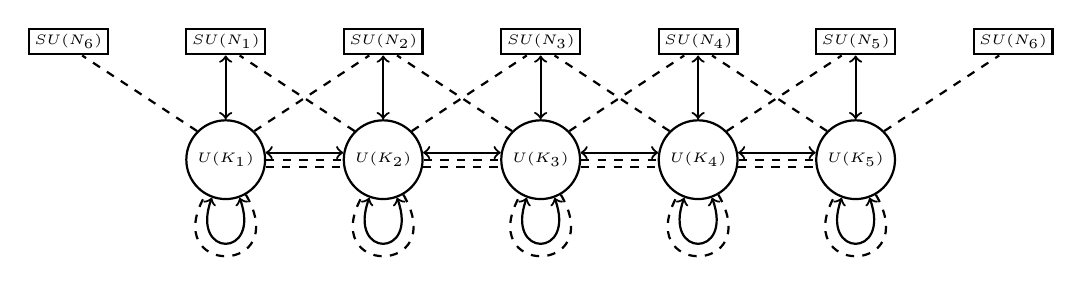
\begin{tikzpicture}[square/.style={regular polygon,regular polygon sides=4},thick,inner sep=0.2em]
    \node(G1) at (0,0)[circle,draw,minimum size=1cm]{\tiny $U(K_1)$};
    \node(F1) at (0,1.5)[draw]{\tiny $SU(N_1)$};
    \draw [<->] (G1.90) to (F1.-90);
    \draw [<->](G1) to [in=250,out=290,looseness=6](G1);
    \draw [dashed](G1) to [in=240,out=300,looseness=6](G1);

    
    \node (G2) at (2,0) [circle,draw,minimum size=1cm]{\tiny $U(K_2)$};
    \node (F2) at (2,1.5)[draw]{\tiny $SU(N_2)$};
    \draw [<->] (G2.90) to (F2.-90);
    \draw [<->] (G2) to [in=250,out=290,looseness=6](G2);        
    \draw [<->] (G1.10) to (G2.170);
    \draw [dashed] (G1.360) to (G2.180);
    \draw [dashed] (G1.350) to (G2.190);
    \draw [dashed](G2) to [in=240,out=300,looseness=6](G2);

    
    \node (G3) at (4,0) [circle,draw,minimum size=1cm]{\tiny $U(K_3)$};
    \node (F3) at (4,1.5)[draw]{\tiny $SU(N_3)$};
    \draw [<->](G3.90) to (F3.-90);
    \draw [<->](G3) to [in=250,out=290,looseness=6](G3);        
    \draw [<->] (G2.10) to (G3.170);
    \draw [dashed] (G2.360) to (G3.180);
    \draw [dashed] (G2.350) to (G3.190);
    \draw [dashed](G3) to [in=240,out=300,looseness=6](G3);
    
    \node (G4) at (6,0) [circle,draw,minimum size=1cm]{\tiny $U(K_4)$};
    \node (F4) at (6,1.5)[draw]{\tiny $SU(N_4)$};
    \draw [<->](G4.90) to (F4.-90);
    \draw [<->](G4) to [in=250,out=290,looseness=6](G4);        
    \draw [<->] (G3.10) to (G4.170);
    \draw [dashed] (G3.360) to (G4.180);
    \draw [dashed] (G3.350) to (G4.190);
    \draw [dashed](G4) to [in=240,out=300,looseness=6](G4);

    \node (G5) at (8,0) [circle,draw,minimum size=1cm]{\tiny $U(K_5)$};
    \node (F5) at (8,1.5)[draw]{\tiny $SU(N_5)$};
    \draw [<->](G5.90) to (F5.-90);
    \draw [<->](G5) to [in=250,out=290,looseness=6](G5);        
    \draw [<->] (G4.10) to (G5.170);
    \draw [dashed] (G4.360) to (G5.180);
    \draw [dashed] (G4.350) to (G5.190);
    \draw [dashed](G5) to [in=240,out=300,looseness=6](G5);
    
    \node (FR) at (10,1.5)[draw]{\tiny $SU(N_6)$};
    \node (FL) at (-2,1.5)[draw]{\tiny $SU(N_6)$};
	
	\draw [dashed] (G1.45) to (F2.225);
	\draw [dashed] (G1.135) to (FL.315);	
	\draw [dashed] (G2.135) to (F1.315);
	\draw [dashed] (G2.45) to (F3.225);
	\draw [dashed] (G3.135) to (F2.315);
	\draw [dashed] (G3.45) to (F4.225);
	\draw [dashed] (G4.135) to (F3.315);
	\draw [dashed] (G4.45) to (F5.225);
	\draw [dashed] (G5.135) to (F4.315);
 	\draw [dashed] (G5.45) to (FR.225);	
  \end{tikzpicture}
  \caption{\it Quiver diagram in $\N=(0,2)$ notation describing M-strings for the $(1,0)_{A_{M-1}}$ theory with $M=6$, $\tilde{\rho}=[N_1,N_2,\dots,N_6]$ and \newline$\tilde{\kappa}=[K_1,K_2,K_3,K_4,K_5,K_6]$, $K_6=0$.}
  \label{fig:ZMquiver}
\end{figure}
In particular
\begin{equation}
\Upsilon\sim \tau\Upsilon\tau^{\dagger}\,,\quad \zeta\sim\tau\zeta\tau^{\dagger}\,,\quad X\sim \tau X\tau^{\dagger}\,,\quad \widetilde{X}\sim\tau\widetilde{X}\tau^{\dagger}\,,\label{eqn:ZM1}
\end{equation}
\begin{equation}
Y\sim \omega\tau Y\tau^{\dagger}\,,\quad \widetilde{Y}\sim \omega^{-1}\tau\widetilde{Y}\tau^{\dagger}\,,\quad \lambda\sim \omega\tau\lambda\tau^{\dagger}\,,\quad \widetilde{\lambda}\sim \omega^{-1}\tau\widetilde{\lambda}\tau^{\dagger}\,,\label{eqn:ZM2}
\end{equation}
\begin{equation}
\phi\sim \tau\phi g^{\dagger}\,,\quad \widetilde{\phi}\sim g\widetilde{\phi}\tau^{\dagger}\,,\quad \psi\sim \omega^{-1}\tau\psi g^{\dagger}\,,\quad \widetilde{\psi}\sim \omega^{-1}g\widetilde{\psi}\tau^{\dagger} \,.\label{eqn:ZM3}
\end{equation}
The field content of the orbifolded theory is then given by solving the  equations \eqref{eqn:ZM1}, \eqref{eqn:ZM2} and \eqref{eqn:ZM3}. The field content is summarised, after setting $k=1$, in Table \ref{tab:d1d5ZMZk}.
From \eqref{eqn:ZM1} we end up with $U(K_n)$, $n=1,\dots, M$ vector multiplets with field strengths $\Upsilon_n$ with chiral multiplets $X_n,\widetilde{X}_n$ and Fermi multiplet $\zeta_n$ all in the adjoint representation of $\mathfrak{u}(K_n)$.
Between each $U(K_n)$ vector multiplet we have chiral multiplets $Y_n$, $\widetilde{Y}_n$ in representations $\mathbf{K}_n\otimes \overline{\mathbf{K}}_{n+1}$, $\mathbf{K}_n\otimes \overline{\mathbf{K}}_{n-1}$ of $\prod_nU\left(K_n\right)$ and Fermi multiplets $\lambda_n,\widetilde{\lambda}_n$ also in representations $\mathbf{K}_n\otimes \overline{\mathbf{K}}_{n+1}$, $\mathbf{K}_n\otimes \overline{\mathbf{K}}_{n-1}$ respectively.
From \eqref{eqn:ZM3} there are Chiral multiplets $\phi_n$, $\widetilde{\phi}_n$ in representations $\mathbf{K}_n\otimes\overline{\mathbf{N}}_n$, $\mathbf{N}_n\otimes\overline{\mathbf{K}}_n$ respectively. There are also Fermi multiplets $\psi_n$, $\widetilde{\psi}_n$ in representations $\mathbf{K}_n\otimes \overline{\mathbf{N}}_{n-1}$, $\mathbf{N}_{n+1}\otimes \overline{\mathbf{K}}_{n}$.
Note that we identify $n\sim n+M$ with the understanding that $K_M=0$.
This can be conveniently summarised in the quiver diagram of Figure \ref{fig:ZMquiver} where circular nodes denote vector multiplets, arrows denote chiral multiplets and dashed lines denote Fermi multiplets.

\subsubsection{D1 Worldvolume Theory \& `Chain-Saw' Quiver}
The theory of M-strings in the presence of the defect is then given by performing a further $\mathbb{Z}_k$ orbifold of the above quiver theory of Figure \ref{fig:ZMquiver}. Since the $\mathbb{Z}_k$ orbifold action preserves the $\N=(0,2)$ supercharges $\Qtwo$, $\widetilde{\Qtwo}$ we may proceed as before. For a $\N=(0,2)$ superfield $f$ in representation $\mathcal{R}:\prod_{n}U(K_n)\times S\prod_nU(N_n)\to \End\mathcal{V}$ the orbifold identifies
\begin{equation}\label{eqn:orbactiongauge}
f\sim \gamma^{J_{12}-J_{710}}\mathcal{R}\left(\tau_1\otimes\dots\otimes\tau_M,g_1\otimes\dots\otimes g_M\right)f\,,
\end{equation}
where 
\begin{align}
&\tau_n=\diag\left(\gamma\mathbb{I}_{K_{n1}},\dots,\gamma^i\mathbb{I}_{K_{ni}},\dots,\gamma^k\mathbb{I}_{K_{nk}}\right)\in U(K_n)\,,\\
&g_n=\gamma^{\frac{1}{2}}\diag\left(\gamma\mathbb{I}_{N_{n1}},\dots,\gamma^i\mathbb{I}_{N_{ni}},\dots,\gamma^k\mathbb{I}_{N_{nk}}\right)\in U(N_n)\,,
\end{align}
corresponding to $\tilde{\rho}_n=[N_{n1},\dots,N_{nk}]$ and $\tilde{\kappa}_n=[K_{n1},\dots,K_{nk}]$.

Note that we also shifted the $\mathbb{Z}_k$ holonomy in $SU(N_n)$ as in \cite{Bullimore:2014upa,Kanno:2011fw}. Explicitly
\begin{equation}
\Upsilon_n\sim \tau_n\Upsilon_n\tau_n^{\dagger}\,,\quad \overline{\xi}_n\sim\gamma\tau_n\overline{\xi}_n\tau_n^{\dagger}\,,\quad X_n\sim \gamma\tau_n X_n\tau_n^{\dagger}\,,\quad \tilde{X}_n\sim\tau_n\tilde{X}_n\tau_n^{\dagger}\,,\label{eqn:Zk1}
\end{equation}
\begin{equation}
Y_n\sim \gamma^{-1}\tau_n Y_n\tau_{n+1}^{\dagger}\,,\quad \tilde{Y}_n\sim \tau_n\tilde{Y}_{n}\tau^{\dagger}_{n-1}\,,\quad \lambda_n\sim \tau_n\lambda_n\tau_{n+1}^{\dagger}\,,\label{eqn:Zk2}
\end{equation}
\begin{equation}
\phi_n\sim \gamma^{\frac{1}{2}}\tau_n\phi_n g_n^{\dagger}\,,\quad \tilde{\lambda}_n\sim \gamma^{-1}\tau_n\tilde{\lambda}_n\tau_{n-1}^{\dagger}\,,
\end{equation}
\begin{equation}
\tilde{\phi}_n\sim \gamma^{\frac{1}{2}}g_n\tilde{\phi}_n\tau_n^{\dagger}\,,\quad \psi_n\sim \gamma^{\frac{1}{2}}\tau_n\psi g_{n-1}^{\dagger}\,,\quad \tilde{\psi}_n\sim \gamma^{\frac{1}{2}}g_{n+1}\tilde{\psi}\tau_n^{\dagger}\,.\label{eqn:Zk3}
\end{equation}
\begin{figure}
\centering
  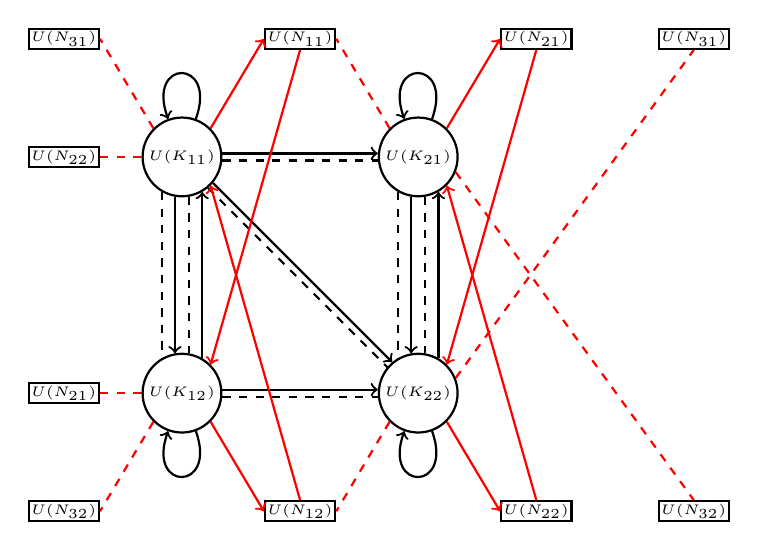
\begin{tikzpicture}[square/.style={regular polygon,regular polygon sides=4},thick,inner sep=0.1em]
  
    %gaugenodes
    \node (G11) at (0,0)[circle,draw,minimum size=1cm]{\tiny $U(K_{11})$};
    \node (G21) at (3,0) [circle,draw,minimum size=1cm]{\tiny $U(K_{21})$};
    \node (G12) at (0,-3)[circle,draw,minimum size=1cm]{\tiny $U(K_{12})$};
    \node (G22) at (3,-3) [circle,draw,minimum size=1cm]{\tiny $U(K_{22})$};

	    
    %adjoint chirals
    \draw [<-] (G11) to [in=70,out=110,looseness=6](G11);
    \draw [<-] (G21) to [in=70,out=110,looseness=6](G21);      
    \draw [->] (G12) to [in=250,out=290,looseness=6](G12);   
    \draw [->] (G22) to [in=250,out=290,looseness=6](G22);   
    
    %X chirals
    \draw [dashed] (G11.240) to (G12.120);
    \draw [->] (G11.260) to (G12.100);
    \draw [dashed] (G11.280) to (G12.80);
    \draw [<-] (G11.300) to (G12.60);

    \draw [dashed] (G21.240) to (G22.120);
    \draw [->] (G21.260) to (G22.100);
    \draw [dashed] (G21.280) to (G22.80);
    \draw [<-] (G21.300) to (G22.60);

    
            
    %tildeY chiral
    \draw [->] (G11.5) to (G21.175);
    \draw [dashed] (G11.355) to (G21.185); 
    \draw [->] (G12.5) to (G22.175);
    \draw [dashed] (G12.355) to (G22.185);
 	
	%Y chiral
    \draw [->] (G11.-40) to (G22.130);
    \draw [dashed] (G11.310) to (G22.140);

    
            
    %flavournodes
    \node (F11) at (1.5,1.5)[draw]{\tiny $U(N_{11})$};
    \node (F21) at (4.5,1.5)[draw]{\tiny $U(N_{21})$};
    \node (F31) at (6.5,1.5)[draw]{\tiny $U(N_{31})$};    
    \node (F12) at (1.5,-4.5)[draw]{\tiny $U(N_{12})$};
    \node (F22) at (4.5,-4.5)[draw]{\tiny $U(N_{22})$};    
    \node (F32) at (6.5,-4.5)[draw]{\tiny $U(N_{32})$};  
    \node (F01) at (-1.5,1.5)[draw]{\tiny $U(N_{31})$};    
    \node (F02) at (-1.5,-4.5)[draw]{\tiny $U(N_{32})$};   
    \node (F22p) at (-1.5,0)[draw]{\tiny $U(N_{22})$};    
    \node (F21p) at (-1.5,-3)[draw]{\tiny $U(N_{21})$};   
    %phi
    \draw [->,color=red] (G11.45) to (F11.180);
    \draw [->,color=red] (G12.-45) to (F12.180);
    \draw [->,color=red] (G22.-45) to (F22.180);
    \draw [->,color=red] (G21.45) to (F21.180);

    
    %tildephi
    \draw [<-,color=red] (G11.-45) to (F12.90);
    \draw [<-,color=red] (G21.-45) to (F22.90);
    \draw [<-,color=red] (G12.45) to (F11.270);
    \draw [<-,color=red] (G22.45) to (F21.270);
    
    %fermions
	\draw [dashed,color=red] (G11.135) to (F01.0);
	\draw [dashed,color=red] (G21.135) to (F11.0);   
	\draw [dashed,color=red] (G12.225) to (F02.0);	
	\draw [dashed,color=red] (G22.225) to (F12.0);
	
	\draw [dashed,color=red] (G11.180) to (F22p.0);  
	\draw [dashed,color=red] (G12.180) to (F21p.0);	
	\draw [dashed,color=red] (G21.-22.5) to (F32.90); 
	\draw [dashed,color=red] (G22.22.5) to (F31.270); 	
  \end{tikzpicture}
  \caption{\it Quiver diagram in $\mathcal{N}=(0,2)$ notation describing $M$-strings for the $(1,0)_{A_{M-1}}$ theory with $M=3$, $k=2$ $MkN=\sum_{n,i}N_{ni}$ and $\tilde{\kappa}_{n=1,2}=[K_{n1},K_{n2}]$, $\tilde{\kappa}_{3}=[0]$. }
  \label{fig:Zkquiver}
\end{figure}
Solving the above equations \eqref{eqn:Zk1}-\eqref{eqn:Zk3} we end up with the field content of Table \ref{tab:d1d5ZMZk}. Namely we have a set of $U\left(K_{ni}\right)$ field strength multiplets $\Upsilon_{ni}$. At each node we have a chiral superfield $\widetilde{X}_{ni}$ in the adjoint. On the other hand along the `$\mathbb{Z}_k$' direction of the quiver nodes are connected by chiral multiplets $X_{ni}$ and Fermi multiplets $\zeta_{ni}$ in $\mathbf{K}_{ni}\otimes\overline{\mathbf{K}}_{n(i+1)}$. 
\begin{table}
\centering
 \begin{tabular}{|c|c|c|c|c|c|c|c|} 
 \hline
 $(0,2)$ & $\prod_{n,i} U(K_{ni})$ & $\prod_{n,i} SU(N_{ni})$& $J_{56}$&$J_L$&$J_R$&$J_L^R$&$J_R^R$\\\hline\hline
$\Upsilon_{ni}$ &adj$_{ni}$ & $\mathbf{1}$&$-\frac{1}{2}$&$0$&$+\frac{1}{2}$&$0$&$-\frac{1}{2}$\\\hline
$\zeta_{ni}$ &\tiny$\yng(1)_{ni}\otimes\overline{\yng(1)}_{n(i+1)}$ & $\mathbf{1}$&$-\frac{1}{2}$&$0$&$-\frac{1}{2}$&$0$&$-\frac{1}{2}$\\\hline
$Y_{ni}$ &\tiny$\yng(1)_{ni}\otimes\overline{\yng(1)}_{(n+1)(i-1)}$ & $\mathbf{1}$&$0$&$0$&$0$&$+\frac{1}{2}$&$+\frac{1}{2}$\\\hline
$\widetilde{Y}_{ni}$ &\tiny$\yng(1)_{ni}\otimes\overline{\yng(1)}_{(n-1)i}$ & $\mathbf{1}$&$0$&$0$&$0$&$-\frac{1}{2}$&$+\frac{1}{2}$\\\hline
$X_{ni}$ & \tiny$\yng(1)_{ni}\otimes\overline{\yng(1)}_{n(i+1)}$ & $\mathbf{1}$&$0$&$-\frac{1}{2}$&$-\frac{1}{2}$&$0$&$0$\\\hline
$\widetilde{X}_{ni}$ &adj$_n$ & $\mathbf{1}$&$0$&$+\frac{1}{2}$&$-\frac{1}{2}$&$0$&$0$\\\hline
$\lambda_{ni}$ &\tiny$\yng(1)_{ni}\otimes\overline{\yng(1)}_{(n+1)i}$ & $\mathbf{1}$&$-\frac{1}{2}$&$-\frac{1}{2}$&$0$&$+\frac{1}{2}$&$0$\\\hline
$\widetilde{\lambda}_{ni}$ &\tiny$\yng(1)_{ni}\otimes\overline{\yng(1)}_{(n-1)(i-1)}$ & $\mathbf{1}$&$-\frac{1}{2}$&$-\frac{1}{2}$&$0$&$-\frac{1}{2}$&$0$\\\hline
$\phi_{ni}$ &\tiny$\yng(1)_{ni}$& \tiny$\overline{\yng(1)}_{ni}$&$0$&$0$&$-\frac{1}{2}$&$0$&$0$\\\hline
$\widetilde{\phi}_{ni}$ &\tiny$\overline{\yng(1)}_{ni}$& \tiny$\yng(1)_{n(i-1)}$&$0$&$0$&$-\frac{1}{2}$&$0$&$0$\\\hline
$\psi_{ni}$ &\tiny$\yng(1)_{ni}$& \tiny$\overline{\yng(1)}_{(n-1)i}$&$-\frac{1}{2}$&$0$&$-\frac{1}{2}$&$0$&$0$\\\hline
$\widetilde{\psi}_{ni}$ &\tiny$\overline{\yng(1)}_{ni}$& \tiny$\yng(1)_{(n+1)(i-1)}$&$-\frac{1}{2}$&$0$&$-\frac{1}{2}$&$0$&$0$\\\hline
\end{tabular}
\caption{\it Gauge covariant field content with $\delta=0$ of the $\N=(4,4)$ vector multiplet $V$.}
 \label{tab:d1d5ZMZk}
\end{table}
In addition there are also the chiral multiplets $Y_{ni}$, $\widetilde{Y}_{ni}$ in $\mathbf{K}_{ni}\otimes\overline{\mathbf{K}}_{(n+1)(i-1)}$, $\mathbf{K}_{ni}\otimes\overline{\mathbf{K}}_{(n-1)i}$ aswell as Fermi multiplets $\lambda_{ni}$, $\widetilde{\lambda}_{ni}$ in $\mathbf{K}_{ni}\otimes\overline{\mathbf{K}}_{(n+1)i}$, $\mathbf{K}_{ni}\otimes\overline{\mathbf{K}}_{(n-1)(i-1)}$. 
Coupling to $SU(N_{ni})$ global symmetries we have chirals $\phi_{ni}$, $\widetilde{\phi}_{ni}$ in representations $\mathbf{K}_{ni}\otimes \overline{\mathbf{N}}_{ni}$, $\mathbf{N}_{n(i-1)}\otimes \overline{\mathbf{K}}_{ni}$ and Fermi multiplets $\psi_{ni}$, $\widetilde{\psi}_{ni}$ in $\mathbf{K}_{ni}\otimes \overline{\mathbf{N}}_{(n-1)i}$, $\mathbf{N}_{(n+1)(i-1)}\otimes \overline{\mathbf{K}}_{ni}$ representations.
The field content can be summarised in the quiver diagram of Figure \ref{fig:Zkquiver}. This is a generalisation of the chainsaw quiver of \cite{Kanno:2011fw}. Circular nodes denote vector multiplets, arrows denote chiral multiplets and dashed lines denote Fermi multiplets. Coloured in red are those, and only those, fields which couple to $U(N_{ni})$ global symmetries. Again we always identify $n\sim n+M$, $i\sim i+k$ and we take $K_{Mi}\equiv0$.

\subsubsection{BPS Equations}
For completeness we list the BPS equations of the 2d gauge system. In other words, the vanishing of the F- and D-term equations. The BPS equations are
\begin{equation}\label{eqn:ADHM}
\phi\overline{\phi}-\overline{\widetilde{\phi}}\widetilde{\phi}+[X,\overline{X}]+[\widetilde{X},\overline{\widetilde{X}}]=\mathfrak{z}\mathbb{I}_K\,,\quad
\phi\widetilde{\phi}+[X,\widetilde{X}]=0\,,
\end{equation}
where here we abuse the notation such that, for example, $X$ denotes the scalar in the $X$ chiral multiplet. We also added in the Fayet-Iliopoulos deformation $\mathfrak{z}$. These are nothing but the ADHM equations for $K$ $U(N)$ instantons. See also Section \ref{Chap:AppInstADHM}. By implementing the projections \eqref{eqn:ZM1}, \eqref{eqn:ZM2}, \eqref{eqn:ZM3}, \eqref{eqn:Zk1}, \eqref{eqn:Zk2} and \eqref{eqn:Zk3} to \eqref{eqn:ADHM} we obtain the BPS equations of the system in the presence of the surface operator
\begin{gather}
\phi_{ni}\overline{\phi}_{ni}-\overline{\widetilde{\phi}}_{ni}\widetilde{\phi}_{ni}+X_{ni}\overline{X}_{n(i+1)}-\overline{X}_{n(i-1)}X_{n(i-1)}+[\widetilde{X}_{ni},\overline{\widetilde{X}}_{ni}]=\mathfrak{z}\mathbb{I}_{K_{ni}}\,,\label{eqn:ADHMZk1}\\
\phi_{ni}\widetilde{\phi}_{n(i+1)}+X_{ni}\widetilde{X}_{n(i+1)}-\widetilde{X}_{ni}X_{ni}=0\,.\label{eqn:ADHMZk2}
\end{gather}

\subsection{BPS Partition Function on \texorpdfstring{$T^2\times\mathbb{R}_{\epsilon_1,\epsilon_2}^4$}{T2 x R4}}
The $T^2\times\mathbb{R}_{\epsilon_1,\epsilon_2}^4$ partition function for the $(1,0)_A$ theories with surface operator labelled by $\rho$ (or equivilently $\tilde{\rho}$) can be defined as the following trace over the Hilbert space $\mathcal{H}$ of the theory \cite{Kim:2017xan,Bhattacharya:2008zy,Kim:2015gha}
\begin{equation}
\begin{aligned}
Z^{\rho}=\Tr_{\mathcal{H}}\Bigg[&(-1)^F\Qtau^{H_-}\overline{\Qtau}^{H_+}\left(\qbf\tbf\right)^{-J_L}\left(\frac{\tbf}{\qbf}\right)^{J_R+J_R^R}\cbf^{2J_L^R}\\
&\times\prod_{n=1}^M\prod_{i=1}^k\left(w_{ni}^{K_{ni}}\prod_{A=1}^{N}x_{ni,A}^{f_{ni,A}}\right)\Bigg]\,.
\end{aligned}
\end{equation}
Here $F=F_-+F_+$ is the fermion number, $H_{\pm}=\frac{1}{2}(H\pm P)$ are the right/left-moving Hamiltonians on $T^2$ and $Q_{\tau}=e^{2\pi\iu\tau}$ is the modular parameter of the torus. Using the 6d supersmmetry generators $\Qsix_{+-}^{\alpha \dot a}$, $\widetilde{\Qsix}_{++}^{\dot\alpha \dot a}$. 
We identify
\begin{equation}
\Qsix:=\widetilde{\Qsix}_{++}^{\dot1 \dot 2}=\Qtwo\,,\quad\widetilde{\Qsix}:=\widetilde{\Qsix}_{++}^{\dot2 \dot 1}=\widetilde{\Qtwo}\,.
\end{equation}
Then, the right-moving Hamiltonian can be written as $H_+=\{\Qsix,\widetilde{\Qsix}\}$ which is also preserved by the surface operator. Since $\Qsix$, $\widetilde{\Qsix}$ commute with $SU(2)_{\alpha}$ and $SU(2)_{a}$ we may include fugacities for their Cartans. Furthermore they commute with the diagonal subgroup $SU(2)_D\subset SU(2)_{\dot\alpha}\times SU(2)_{\dot a}$ hence we also include a fugacity for its Cartan $J_D=J_R+J^R_R$. We also include fugacities $x_{ni,A}$ for the Cartans $f_{ni,A}$ of $\mathfrak{u}(N_{ni})$. We also include fugacity $w_{in}$ for the string winding number $K_{ni}$. Moreover, $\qbf,\tbf,\cbf$ are related to the torus action $U(1)_{\epsilon_1}\times U(1)_{\epsilon_2}\times U(1)_{m}$ of \eqref{eqn:omegaback}, \eqref{eqn:massback} on $\mathbb{C}^3$ by
\begin{equation}
\qbf=e^{2\pi\iu\epsilon_1}\,,\quad \tbf=e^{-2\pi\iu\epsilon_2}\,,\quad \cbf=e^{2\pi\iu m}\,.
\end{equation}
The partition function $Z$ counts states annihilated by both $\Qsix$ and $\widetilde{\Qsix}$. In particular it factorises as
\begin{equation}\label{eqn:Zstringdef1}
Z^{\rho}=Z^{\rho}_{\text{pert}}Z^{\rho}_{\text{string}}\,,\quad Z^{\rho}_{\text{string}}=\sum_{\substack{K_{ni}\geq0\\K_{Mi}=0}}\left(\prod_{n=1}^M\prod_{i=1}^kw_{ni}^{K_{ni}}\right)\Ell^{\tilde{\rho}}_{\tilde{\kappa}=[K_{11},\dots,K_{Mk}]}
\end{equation}
where $Z_{\text{pert}}$ is the contribution from the BPS particles. Due to the $\Omega$-background the BPS strings are localised to sit at the origin of $\mathbb{R}^4_{\epsilon_1,\epsilon_2}$ and wrap the $T^2$. This gives rise to the effective 2d description that we described in the previous section. $\Ell^{\tilde{\rho}}_{\tilde{\kappa}}$ is the Elliptic genus partition function, which will be defined in Section \ref{sec:nodefect}, of said 2d theory and $\Ell^{\tilde{\rho}}_{[0,0,\dots,0]}\equiv1$.
\begin{table}
\centering
 \begin{tabular}{|c|c|c|c|c|c|c|} 
 \hline
  & & $\mathfrak{su}(2)_L$ & $\mathfrak{su}(2)_R$& $\mathfrak{su}(2)_R^R$&$\mathfrak{u}(1)_{H_-}$&$i$\\\hline\hline
\multirow{2}{*}{Half-Hyper}&$\phi$ &$\mathbf{1}$ & $\mathbf{1}$&$\mathbf{2}$&$0$&$\sqrt{\frac{\qbf}{\tbf}}+\sqrt{\frac{\tbf}{\qbf}}$\\
&$\psi$ &$\mathbf{2}$ & $\mathbf{1}$&$\mathbf{1}$&$0$&$-\sqrt{\qbf\tbf}-\sqrt{\frac{1}{\qbf\tbf}}$\\\hline
\multirow{3}{*}{Tensor}&$\sigma$ &$\mathbf{1}$ & $\mathbf{1}$&$\mathbf{1}$&$0$&$1$\\
&$\lambda$ &$\mathbf{2}$ & $\mathbf{1}$&$\mathbf{2}$&$0$&$-\qbf-\tbf-\frac{1}{\qbf}-\frac{1}{\tbf}$\\
&$B$ &$\mathbf{3}$ & $\mathbf{1}$&$\mathbf{1}$&$0$&$\qbf\tbf+1+\frac{1}{\tbf\qbf}$\\\hline\hline
&$\partial_{\alpha\dot\alpha}$ &$\mathbf{2}$ & $\mathbf{2}$&$\mathbf{1}$&$0$&$\qbf,\tbf,\frac{1}{\qbf},\frac{1}{\tbf}$\\
&$\partial_{-}$ &$\mathbf{2}$ & $\mathbf{1}$&$\mathbf{1}$&$1$&$\Qtau$\\\hline
\end{tabular}
\caption{\it Letters contributing to $Z^{\rho}_{\text{pert}}$.}\label{tab:6dletter}
\end{table}
The perturbative piece is given by enumerating all letters of Table \ref{tab:6dletter} \cite{Kim:2017xan,Kim:2015gha}, for the case without defect $\rho=\emptyset$ it reads
\begin{align}
&\label{eqn:pertpi}Z^{\rho=\emptyset}_{\text{pert}}=\PE\left[i\right]\,,\quad i=\frac{\left(i_{\text{hyp}}+i_{\text{Tensor}}\right)\qbf\tbf}{(1-\Qtau)(1-\qbf)^2(1-\tbf)^2}\\
&i_{\text{hyp}}= \left(\sqrt{\frac{\qbf}{\tbf}}+\sqrt{\frac{\tbf}{\qbf}}-\sqrt{\qbf\tbf}-\sqrt{\frac{1}{\qbf\tbf}}\right)\left(\cbf+\cbf^{-1}\right)\sum_{n=1}^M\sum_{A=1}^Nx_{n,A}x_{n+1,B}^{-1}\\
&i_{\text{Tensor}}= NM\left(2+\qbf\tbf+\frac{1}{\tbf\qbf}-\qbf-\tbf-\frac{1}{\qbf}-\frac{1}{\tbf}\right)\,.
\end{align}
We can also compute the perturbative piece for the $T^2\times\mathbb{R}^4_{\epsilon_1,\epsilon_2}$ partition function for the theory in the presence of the defect by performing the orbifolding procedure to the letters of Table \ref{tab:6dletter}. 
\begin{align}
&\label{eqn:pertpiorb}Z^{\rho}_{\text{pert}}=\PE\left[i^{\text{orb}}\right]\,,\quad i^{\text{orb}}=\frac{1}{|\mathbb{Z}_k|}\sum_{\gamma\in\mathbb{Z}_k}\frac{\left(i^{\text{orb}}_{\text{hyp}}+i^{\text{orb}}_{\text{Tensor}}\right)\gamma\qbf\tbf}{(1-\Qtau)(1-\gamma\qbf)^2(1-\tbf)^2}\\
&\begin{aligned}i^{\text{orb}}_{\text{hyp}}=& \left(\gamma\sqrt{\frac{\qbf}{\tbf}}+\sqrt{\frac{\tbf}{\qbf}}-\gamma\sqrt{\qbf\tbf}-\sqrt{\frac{1}{\qbf\tbf}}\right)\left(\frac{\cbf}{\gamma}+\frac{1}{\cbf}\right)\\
&\times\sum_{i,j=1}^k\sum_{n=1}^M\sum_{A=1}^{N_{ni}}\sum_{B=1}^{N_{(n+1)j}}\frac{\gamma^{i-j}x_{ni,A}}{x_{(n+1)j,B}}\end{aligned}\\
&i^{\text{orb}}_{\text{Tensor}}= NM\left(2+\gamma\tbf\qbf+\frac{\gamma}{\tbf\qbf}-\gamma\qbf-\tbf-\frac{\gamma}{\qbf}-\frac{1}{\tbf}\right)\,.
\end{align}
\subsection{M-String Elliptic Genus Without Surface Operator}\label{sec:nodefect}
We now turn towards computing the supersymmetric index a.k.a flavoured elliptic genus partition function for our theory. In this section we begin by reviewing the index computation for the case without surface operator $(k=1)$ i.e $K$ M-strings inside $M$ M5-branes sitting at the tip of a $A_{N-1}$ singularity without surface operator. Following that we compute the M-string elliptic genus partition function with the surface operator.

This index may be viewed either as a path integral of the theory on $T^2$ in which case it may be computed from localisation techniques \cite{Benini:2013nda,Benini:2013xpa} or, since our theory admits a free field limit, as a counting problem on $T^2$ in the radial quantisation in which case it may be computed via `letter counting' \cite{Putrov:2015jpa,Gadde:2013wq,Gadde:2013ftv,Gadde:2014ppa,Gadde:2013lxa,Nakayama:2011pa,Cordova:2017ohl,Bourton:2017pee}. 

The elliptic genus for a fixed string number configuration \newline $\tilde{\kappa}=[K_1,K_2,\dots,K_{M-1},K_M=0]$ and $\tilde{\rho}=[N_1,\dots,N_M]$ is then defined to be  
\begin{equation}\label{eqn:Ellnodefect}
\begin{aligned}
\Ell^{\tilde{\rho}}_{\tilde{\kappa}}&(\Qtau,\qbf,\tbf,\mathbf{c},\vec{x}_{n})=\\ &\Tr_{\text{R}}\left[(-1)^F\Qtau^{H_-}\left(\qbf\tbf\right)^{-J_L}\left(\frac{\tbf}{\qbf}\right)^{J_R+J_R^R}\cbf^{2J_L^R}\prod_{n=1}^M\prod_{A=1}^{N}x_{n,A}^{f_{n,A}}\right]\,.
\end{aligned}
\end{equation}
Here $F=F_-+F_+$ is the fermion number and the trace is taken over the Hilbert space on $\mathbb{S}^1$ in the radial quantisation. 
The full index is then given by
\begin{equation}
\Ell^{\tilde{\rho}}_{\tilde{\kappa}}(\Qtau,\qbf,\tbf,\mathbf{c},\vec{x}_{n})=\prod_{n=1}^M\frac{1}{K_n!}\oint\prod_{I=1}^{K_n}\frac{dy_{n,I}}{2\pi\iu y_{n,I}}\prod_{P}\mathcal{\Ell}_{P}(\Qtau,\qbf,\tbf,\cbf,\vec{x}_{n},\vec{y}_{n})
\end{equation}
where the product over $P$ denotes the product over all $\N=(0,2)$ multiplets of the theory and $\Ell_P$ their contributions to the index, which are listed in Appendix \ref{App:Ell}. It is convenient to rewrite the index as
\begin{equation}\label{eqn:Ellnodefectcont}
\Ell^{\tilde{\rho}}_{\tilde{\kappa}}=\prod_{n=1}^M\frac{1}{K_n!}\oint\prod_{I=1}^{K_n}\frac{dy_{n,I}}{2\pi\iu y_{n,I}}\Ell^{\text{tens}}_{\tilde{\kappa}}\Ell^{\text{hyp}}_{\tilde{\kappa}}\,;
\end{equation}
we have divided up the corresponding contributions from 6d $\mathcal{N}=(1,0)$ tensor multiplets (uncharged under $\cbf$)
\begin{equation}
\begin{aligned}
\Ell^{\text{tens}}_{\tilde{\kappa}}=&\prod_{P\in\{\Upsilon,\zeta,X,\widetilde{X},\phi,\widetilde{\phi}\}}\Ell_{\mathcal{M}}\\
=&\prod_{n=1}^{M}\left(\iu\eta(\Qtau)\right)^{3K_n}\frac{\prod_{I\neq J}\theta_1\left(\frac{y_{n,I}}{y_{n,J}};\Qtau\right)\prod_{I,J=1}^{K_n}\theta_1\left(\frac{\qbf}{\tbf}\frac{y_{n,I}}{y_{n,J}};\Qtau\right)}{\prod_{I,J=1}^{K_n}\theta_1\left(\tbf^{-1}\frac{y_{n,I}}{y_{n,J}};\Qtau\right)\theta_1\left(\qbf\frac{y_{n,I}}{y_{n,J}};\Qtau\right)}\\
&\times\prod_{n=1}^M\prod_{I=1}^{K_n}\prod_{A=1}^N\frac{(\iu\eta(\Qtau))^2}{\theta_1\left(\sqrt{\frac{\qbf}{\tbf}}\frac{x_{n,A}}{y_{n,I}};\Qtau\right)\theta_1\left(\sqrt{\frac{\qbf}{\tbf}}\frac{y_{n,I}}{x_{n,A}};\Qtau\right)}
\end{aligned}
\end{equation}
and $\mathcal{N}=(1,0)$ hypermultiplets (charged under $\cbf$)
\begin{equation}
\begin{aligned}
&\Ell^{\text{hyp}}_{\tilde{\kappa}}=\prod_{P\in\{\lambda,\widetilde{\lambda},Y,\widetilde{Y},\psi,\widetilde{\psi}\}}\Ell_{P}\\
=&\prod_{n=1}^{M}\prod_{I=1}^{K_n}\frac{\prod_{J=1}^{K_{n-1}}\theta_1\left(\cbf\sqrt{\frac{1}{\qbf\tbf}}\frac{y_{n-1,J}}{y_{n,I}};\Qtau\right)\prod_{J=1}^{K_{n+1}}\theta_1\left(\cbf^{-1}\sqrt{\frac{1}{\qbf\tbf}}\frac{y_{n+1,J}}{y_{n,I}};\Qtau\right)}{\prod_{J=1}^{K_{n-1}}\theta_1\left(\cbf^{-1}\sqrt{\frac{\tbf}{\qbf}}\frac{y_{n,I}}{y_{n-1,J}};\Qtau\right)\prod_{J=1}^{K_{n+1}}\theta_1\left(\cbf\sqrt{\frac{\qbf}{\tbf}}\frac{y_{n,I}}{y_{n+1,J}};\Qtau\right)}\\
&\times\prod_{n=1}^{M}\prod_{I=1}^{K_n}\prod_{A=1}^N\frac{\theta_1\left(\cbf\frac{x_{n-1,A}}{y_{n,I}};\Qtau\right)\theta_1\left(\mathbf{c}\frac{y_{n,I}}{x_{n+1,A}};\Qtau\right)}{(\iu\eta(\Qtau))^2}\,.
\end{aligned}
\end{equation}
See Appendix \ref{App:EllipticGenus} for the definition of the $\theta_1$ function and various properties. We identify $n\sim n+M$ orbifold indices within the products. The countour integrals \eqref{eqn:Ellnodefectcont} should be computed using the Jefferey-Kirwan residue prescription \cite{1993alg.geom..7001J,Benini:2013nda,Benini:2013xpa}. 
Equation \eqref{eqn:Ellnodefect} may be expressed as a sum of residues associated to poles classified by $M$ $N$-coloured Young's diagrams $\vec{\mu}_n$ such that $|\vec{\mu}_n|:=\sum_{A}|\mu_{n,A}|=K_n$. We choose the $+\sum y$ JK prescription. The pole corresponding to the box $s=(l,p)\in\mu_{n,A}$ is then
\begin{equation}\label{eqn:polekeep}
y_n(s)=x_{n,A}\qbf^{l-\frac{1}{2}}\tbf^{-p+\frac{1}{2}}\,.
\end{equation}
As explained in \cite{Kim:2011mv,Kim:2012gu} only residues arising from these poles should be kept. We also assumed that the $x$'s can be made sufficiently generic. The residue for a fixed coloured Young diagram is then 
\begin{equation}\label{eqn:Mstringyng}
\Ell^{\tilde{\rho}}_{\tilde{\kappa},\vec{\mu}_n}=\Ell_{\tilde{\kappa},\vec{\mu}_n}^{\text{tens}}\Ell_{\tilde{\kappa},\vec{\mu}_n}^{\text{hyp}}
\end{equation}
where
\begin{equation}
\begin{aligned}
&\Ell_{\tilde{\kappa},\vec{\mu}_n}^{\text{tens}}=\prod_{n=1}^M\prod_{A,B=1}^{N}\left\{\prod_{\substack{(l_1,p_1)\in \mu_{{n,A}}\\(l_2,p_2)\in \mu_{{n,B}}}}\frac{\theta_1\left(\qbf^{l_1-l_2}\tbf^{-p_1+p_2}\frac{x_{n,A}}{x_{n,B}};\Qtau\right)}{\theta_1\left(\qbf^{l_1-l_2}\tbf^{-p_1+p_2-1}\frac{x_{n,A}}{x_{n,A_2}};\Qtau\right)}\right.\\
&\prod_{\substack{(l_1,p_1)\in \mu_{{n,A}}\\(l_2,p_2)\in \mu_{{n,B}}}}\frac{\theta_1\left(\qbf^{l_1-l_2}\tbf^{-p_1+p_2}\frac{\qbf}{\tbf}\frac{x_{n,A}}{x_{n,B}};\Qtau\right)}{\theta_1\left(\qbf^{l_1-l_2+1}\tbf^{-p_1+p_2}\frac{x_{n,A}}{x_{n,B}};\Qtau\right)}\\
&\left.\prod_{(l,p)\in \mu_{n,B}}\frac{1}{\theta_1\left(\qbf^{-l+1}\tbf^{p-1}\frac{x_{n,A}}{x_{n,B}};\Qtau\right)\theta_1\left(\qbf^{l}\tbf^{-p}\frac{x_{n,B}}{x_{n,A}};\Qtau\right)}\right\}\,,
\end{aligned}
\end{equation}
and
\begin{equation}
\begin{aligned}
&\Ell_{\tilde{\kappa},\vec{\mu}_n}^{\text{hyp}}=\prod_{n=1}^M\prod_{A,B=1}^{N}\Bigg\{\prod_{\substack{(l_1,p_1)\in \mu_{{n,A}}\\(l_2,p_2)\in \mu_{{n-1,B}}}}\frac{\theta_1\left(\cbf^{-1}\qbf^{l_1-l_2-\frac{1}{2}}\tbf^{-p_1+p_2-\frac{1}{2}}\frac{x_{n,A}}{x_{n-1,B}};\Qtau\right)}{\theta_1\left(\cbf\qbf^{-l_1+l_2-\frac{1}{2}}\tbf^{p_1-p_2+\frac{1}{2}}\frac{x_{n-1,B}}{x_{n,A}};\Qtau\right)}\\
&\prod_{\substack{(l_1,p_1)\in \mu_{{n,A}}\\(l_2,p_2)\in \mu_{{n-1,B}}}}\frac{\theta_1\left(\cbf\qbf^{-l_1+l_2-\frac{1}{2}}\tbf^{p_1-p_2-\frac{1}{2}}\frac{x_{n-1,B}}{x_{n,A}};\Qtau\right)}{\theta_1\left(\cbf^{-1}\qbf^{l_1-l_2-\frac{1}{2}}\tbf^{-p_1+p_2+\frac{1}{2}}\frac{x_{n,A}}{x_{n-1,B}};\Qtau\right)}\\
&\prod_{(l,p)\in \mu_{n,B}}\theta_1\left(\cbf\qbf^{-l+\frac{1}{2}}\tbf^{p-\frac{1}{2}}\frac{x_{n-1,A}}{x_{n,B}};\Qtau\right)\theta_1\left(\cbf\qbf^{l-\frac{1}{2}}\tbf^{-p+\frac{1}{2}}\frac{x_{n,B}}{x_{n+1,A}};\Qtau\right)\Bigg\}\,.
\end{aligned}
\end{equation}
Note that the above function contains various factors of $\theta_1(1;\Qtau)$ albeit which cancel between numerator and denominator, thus rendering \eqref{eqn:Mstringyng} well defined. Equation \eqref{eqn:Mstringyng} may be simplified by means of the identity \eqref{eqn:youngsimp} where the sums over monomials are translated into products over Jacobi theta functions. Hence we may write \eqref{eqn:Mstringyng} as
\begin{equation}
\begin{aligned}
\Ell^{\tilde{\rho}}_{\tilde{\kappa},\vec{\mu}_n}=\prod_{n=1}^M&\prod_{A,B=1}^{N}\prod_{(l,p)\in \mu_{{n,A}}}\left\{\frac{\theta_1\left(\cbf\qbf^{l-\mu_{n-1,B;p}^{\trans}-\frac{1}{2}}\tbf^{-\mu_{n,A;l}-\frac{1}{2}+p}\frac{x_{n-1,B}}{x_{n,A}};\Qtau\right)}{\theta_1\left(\qbf^{l-\mu_{n,B;p}^{\trans}}\tbf^{-1-\mu_{n,A;l}+p}\frac{x_{n,A}}{x_{n,B}};\Qtau\right)}\right.\\
&\left.\times\frac{\theta_1\left(\cbf\qbf^{\mu^{\trans}_{n+1,B;p}-l+\frac{1}{2}}\tbf^{-p+\mu_{n,A;l}+\frac{1}{2}}\frac{x_{n,A}}{x_{n+1,B}};\Qtau\right)}{\theta_1\left(\qbf^{1+\mu^{\trans}_{n,B;p}-l}\tbf^{-p+\mu_{n,A;l}}\frac{x_{n,B}}{x_{n,A}};\Qtau\right)}\right\}\,.\\
\end{aligned}
\end{equation}
Summing over all coloured Young diagrams $\vec{\mu}_n$ with exactly $K_n$ boxes means equation \eqref{eqn:Ellnodefect} reads
\begin{equation}\label{eqn:6dpartitionfunctionyng}
\Ell^{\tilde{\rho}}_{\tilde{\kappa}}(\Qtau,\qbf,\tbf,\cbf,\vec{x}_{n}):=\sum_{\substack{\vec{\mu}_{n}\\|\vec{\mu}_n|=K_n}}\Ell^{\tilde{\rho}}_{\tilde{\kappa},\vec{\mu}_n}(\Qtau,\qbf,\tbf,\cbf,\vec{x}_{n})\,.
\end{equation}
The grand partition function obtained by `integrating' over all partitions $\tilde{\kappa}$ which we weight by fugacity $w_n$ ($w_M=0$ to enforce $K_M=0$) is then the total self dual-string contribution to the partition function:
\begin{equation}\label{eqn:6dpartitionfunction}
Z^{\rho}_{\text{string}}(\Qtau,\qbf,\tbf,\cbf,\vec{x}_{n};w_n):=\sum_{\vec{\mu}_{n}}\left(\prod_{n=1}^Mw_{n}^{|\vec{\mu}_n|}\right)\Ell^{\tilde{\rho}}_{\tilde{\kappa},\vec{\mu}_n}(\Qtau,\qbf,\tbf,\cbf,\vec{x}_{n})\,.
\end{equation}
Considering \eqref{eqn:6dpartitionfunction} as a generating function for the partition functions of a $\tilde{\kappa}$ M-string configurations in which case $w_n=e^{2\pi\iu t_{n,n+1}}$ is related to the separation between the $n^{\text{th}}$ and $(n+1)^{\text{th}}$ M5-brane \eqref{eqn:stringtension} \cite{Haghighat:2013tka}. It was demonstrated in \cite{Haghighat:2013tka} that \eqref{eqn:6dpartitionfunction}, combined with the perturbative piece \eqref{eqn:pertpi} reproduces the worldvolume theory of $M$ M5-branes on a transverse $A_{N-1}$ singuarity, as computed using the refined topological vertex.

\subsection{M-String Elliptic Genus With Surface Operator}
We now turn to the case with defect. The partition function we compute is equivalent to the K-theoretic version of the one computed in \cite{Kanno:2011fw} further generalised to quiver theory with flavour. The elliptic genus for the theory of defect M-strings is defined in mostly the same way as before. The only difference in the definition is that we now have fugacities $\vec{x}_{ni}$ for the Cartans $f_{ni}$ of $\mathfrak{u}\left(N_{ni}\right)$. For a fixed string partition $\tilde{\kappa}$ we have
\begin{equation}\label{eqn:indexdefect}
\begin{aligned}
\Ell^{\tilde{\rho}}_{\tilde{\kappa}}&(\Qtau,\qbf,\tbf,\cbf,\vec{x}_{ni})=\\
&\Tr_{\text{R}}\left[(-1)^Fq^{H_-}\left(\qbf\tbf\right)^{-J_L}\left(\frac{\qbf}{\tbf}\right)^{-J_R-J_R^R}\cbf^{2J_L^R}\prod_{n,i}\prod_{A=1}^{N_{ni}}x_{ni,A}^{f_{ni,A}}\right]\,.
\end{aligned}
\end{equation}
The elliptic genus then takes the form
\begin{equation}\label{eqn:contourdefect}
\begin{aligned}
\Ell^{\tilde{\rho}}_{\tilde{\kappa}}(\Qtau,\qbf,&\tbf,\cbf,\vec{x}_{ni}):=\\
&\prod_{n=1}^M\prod_{i=1}^k\frac{1}{K_{ni}!}\oint\prod_{I=1}^{K_{ni}}\frac{dy_{ni,I}}{2\pi\iu y_{ni,I}}\prod_{P}\Ell^{\mathbb{Z}_k}_{P}(\Qtau,\qbf,\tbf,\cbf,\vec{x}_{ni},\vec{y}_{ni})\,,
\end{aligned}
\end{equation}
where the 1-loop determinants $\Ell_{P}^{\mathbb{Z}_k}$ for each multiplet $P$ is given in Appendix \ref{App:EllZk}. At the level of the elliptic genus the orbifold action \eqref{eqn:orbaction}, \eqref{eqn:orbactiongauge} in the IIB description may be traded for an action on the fugacities
\begin{equation}\label{eqn:orbfugacity}
\mathbb{Z}_k:\qbf\mapsto \gamma\qbf\,,\quad \cbf^2\mapsto \gamma^{-1}\cbf^2\,,\quad \vec{x}_{ni}\mapsto \gamma^{i+\frac{1}{2}}\vec{x}_{ni}\,,\quad \vec{y}_{ni}\mapsto \gamma^i\vec{y}_{ni}\,,
\end{equation}
with trivial action on all other fugacties.
As before, the terms attributed to 6d $\mathcal{N}=(1,0)$ tensor multiplets are uncharged under the $\cbf$ fugacity while those coming from $(1,0)$ hypermultiplets are charged under $\cbf$.
We may now perform the integrals. After the orbifolding the solutions are again labelled by $M$ $N$-tuples of Youngs diagrams $\vec{\mu}_n=\{\mu_{ni,A}\}$ with $n=1,\dots,M$ $i=1,\dots,k$ and $A=1,\dots, N_{ni}$. Each $N$-tuple has $|\vec{\mu}_n|=\sum_{i=1}^kK_{ni}=K_{n}$. For a box $s=\left(l,p\right)\in \mu_{ni,A}$ in the $+\sum y$ JK-prescription the corresponding pole is given by
\begin{equation}\label{eqn:res}
y_{nj}(s)=x_{ni,A}\qbf^{l-\frac{1}{2}}\tbf^{-p+\frac{1}{2}}|_{i+l=j\bmod k}\,
\end{equation}
i.e. the $\mathbb{Z}_{k}$ invariant part of \eqref{eqn:polekeep}. In \cite{Gorsky:2017hro} the contour integral representation for the partition function of $\mathbb{C}\times\mathbb{C}/\mathbb{Z}_k$ instantons for 4d $\N=2$ theories was analysed in detail. It was shown that to evaluate the contour integral is equivalent to projecting onto $\mathbb{Z}_k$ invariant terms in the original Nekrasov expression. As in the case without surface operator, the partition function \eqref{eqn:contourdefect} may be thought of as the elliptic uplift of \cite{Gorsky:2017hro}. Hence our integrals may be computed by projecting onto the $\mathbb{Z}_k$ invariant parts of \eqref{eqn:Mstringyng}. The string number $K_{ni}$ for each factor in $\prod_{n,i}U(N_{ni})$ is hence given by the height of the $l^{\text{th}}$ row in a given $\mu_{ni,A}$ and then summing over all contributions
\begin{equation}\label{eqn:Kni}
K_{nj}=K_{nj}(\vec{\mu}_{ni})=\sum_{l=0}^{\infty}\sum_{A=1}^{N_{n(i+1-l)}}\mu^{\trans}_{n(i+1-l),A;l}\,.
\end{equation}
The $\mathbb{Z}_k$ invariant part of \eqref{eqn:6dpartitionfunctionyng} is \cite{Gorsky:2017hro,Kanno:2011fw} \footnote{Upon taking a decoupling limit where we discard all $\theta_1$ which depend on $\cbf$ and then take, for example $N_{(n=1)i}=N_i$, $N_{(n\neq 1)i}=0$ \eqref{eqn:defectyngtens} is to be compared with the elliptic version of equation (2.43) of \cite{Kanno:2011fw}. Sending back $\epsilon_2^{\text{them}}/k\mapsto\epsilon_2^{\text{them}}$ and $\epsilon_1^{\text{them}}\leftrightarrow\epsilon_2^{\text{them}}$ then our parameters are related (up to various factors of $2\pi\iu$) by $x_{1i,A}\sim e^{i\epsilon_1^{\text{them}}-a^{\text{them}}_{A,i}}$, $\tbf^{-1}\sim e^{\epsilon_1^{\text{them}}}$, $\qbf\sim e^{\epsilon_2^{\text{them}}}$.} 
\begin{equation}
\Ell_{\tilde{\kappa},\vec{\mu}_{ni}}^{\tilde{\rho}}=\Ell_{\tilde{\kappa},\vec{\mu}_{ni}}^{\text{tens}}\Ell_{\tilde{\kappa},\vec{\mu}_{ni}}^{\text{hyp}}
\end{equation}
where the contribution from tensor multiplets is
\begin{align*}\label{eqn:defectyngtens}\allowdisplaybreaks
&\Ell_{\tilde{\kappa},\vec{\mu}_{ni}}^{\text{tens}}=\prod_{n=1}^M\prod_{u,i,j=1}^k\prod_{\substack{{A_1,A_2=1}\\(kl_1+i,p_1)\\(kl_2+j,p_2)}}^{N_{n(u-i+1)},N_{n(u-j+1)}}\frac{\theta_1\left(\qbf^{\gamma_{ij}}\tbf^{-p_1+p_2}\frac{x_{n(u-i+1),A_1}}{x_{n(u-j+1),A_2}};\Qtau\right)}{\theta_1\left(\qbf^{\gamma_{ij}}\tbf^{-p_1+p_2-1}\frac{x_{n(u-i+1),A_1}}{x_{n(u-j+1),A_2}};\Qtau\right)}\\
&\times\prod_{n=1}^M\prod_{u,i,j=1}^k\prod_{\substack{{A_1,A_2=1}\\(kl_1+i,p_1)\\(kl_2+j,p_2)}}^{N_{n(u-i)},N_{n(u-j+1)}}\frac{\theta_1\left(\qbf^{\gamma_{(i+1)j}}\tbf^{-p_1+p_2-1}\frac{x_{n(u-i),A_1}}{x_{n(u-j+1),A_2}};\Qtau\right)}{\theta_1\left(\qbf^{\gamma_{(i+1)j}}\tbf^{-p_1+p_2}\frac{x_{n(u-i),A_1}}{x_{n(i-j+1),A_2}};\Qtau\right)}\\
&\times\prod_{n=1}^M\prod_{i,j=1}^k\prod\limits_{A=1}^{N_{ni}}\frac{1}{\prod\limits_{\substack{{B=1}\\(lk+j,p)}}^{N_{n(i-j+1)}}\theta_1\left(\qbf^{-\gamma_j}\tbf^{-1+p}\frac{x_{ni,A}}{x_{n(i-j+1),B}};\Qtau\right)}\\
&\times\prod_{n=1}^M\prod_{i,j=1}^k\prod\limits_{A=1}^{N_{ni}}\frac{1}{\prod\limits_{\substack{{B=1}\\(kl+j,p)}}^{{N_{n(i-j)}}}\theta_1\left(\qbf^{\gamma_{j+1}}\tbf^{-p}\frac{x_{n(i-j),B}}{x_{ni,A}};\Qtau\right)}\,.
\end{align*}
and, from hypers,
\begin{align*}\allowdisplaybreaks
&\Ell_{\tilde{\kappa},\vec{\mu}_{ni}}^{\text{hyp}}=\prod_{n=1}^M\prod_{i,j=1}^k\Bigg\{\prod\limits_{A=1}^{N_{(n-1)i}}\prod\limits_{\substack{B=1\\(kl+j,p)}}^{N_{n(i-j)}}\theta_1\left(\cbf\qbf^{-\gamma_{j+1}+\frac{1}{2}}\tbf^{p-\frac{1}{2}}\frac{x_{(n-1)i,A}}{x_{n(i-j),B}};\Qtau\right)\\
&\prod_{u=1}^k\frac{\prod\limits_{\substack{A_1,A_2=1\\(kl_1+i,p_1)\\(kl_2+j,p_2)}}^{N_{(n-1)(u-i+1)},N_{n(u-j)}}\theta_1\left(\cbf\qbf^{\gamma_{i(j+1)}+\frac{1}{2}}\tbf^{-p_1+p_2-\frac{1}{2}}\frac{x_{(n-1)(u-i+1),A_1}}{x_{n(u-j),A_2}};\Qtau\right)}{\prod\limits_{\substack{A_1,A_2=1\\(kl_1+i,p_1)\\(kl_2+j,p_2)}}^{N_{n(u-i+1)}N_{(n-1)(u-j+1)}}\theta_1\left(\cbf^{-1}\qbf^{\gamma_{ij}-\frac{1}{2}}\tbf^{-p_1+p_2+\frac{1}{2}}\frac{x_{n(u-i+1),A_1}}{x_{(n-1)(u-j+1),A_2}};\Qtau\right)}\\
&\times\prod_{u=1}^k\frac{\prod\limits_{\substack{A_1,A_2=1\\(kl_1+i,p_1)\\(kl_2+j,p_2)}}^{N_{(n+1)(u-i+1)},N_{n(u-j+1)}}\theta_1\left(\cbf\qbf^{\gamma_{ij}-\frac{1}{2}}\tbf^{-p_1+p_2-\frac{1}{2}}\frac{x_{n(u-i+1),A_1}}{x_{(n+1)(u-j+1),A_2}};\Qtau\right)}{\prod\limits_{\substack{A_1,A_2=1\\(kl_1+i,p_1)\\(kl_2+j,p_2)}}^{N_{n(u-i+1)},N_{(n+1)(u-j)}}\theta_1\left(\cbf\qbf^{\gamma_{i(j+1)}+\frac{1}{2}}\tbf^{-p_1+p_2+\frac{1}{2}}\frac{x_{n(u-i+1),A_1}}{x_{(n+1)(u-j),A_2}};\Qtau\right)}\\
&\times\prod\limits_{A=1}^{N_{(n+1)i}}\prod\limits_{\substack{B=1\\(kl+j,p)}}^{N_{n(i-j+1)}}\theta_1\left(\cbf\qbf^{\gamma_{j}+\frac{1}{2}}\tbf^{-p+\frac{1}{2}}\frac{x_{n(i-j+1),B}}{x_{(n+1)i),A}};\Qtau\right)\Bigg\}\,,
\end{align*}
and we understand
\begin{gather}
\gamma_j:=-k\floork{i-j}+j-1+kl\,,\\\gamma_{ij}:=-k\floork{u-i}+k\floork{u-j}+i-j+k(l_1-l_2)\,,
\end{gather}
within the products, where $\left\lfloor\cdot\right\rfloor$ is the floor function. For the sake of compactness we write
\begin{equation}
\prod\limits_{\substack{{A,B=1}\\(l_1,p_1)\in \mu_{ni,A}\\(l_2,p_2)\in \mu_{mj,B}}}^{N_{ni},N_{mj}}\equiv\prod\limits_{A=1}^{N_{ni}}\prod\limits_{B=1}^{N_{mj}}\prod\limits_{(l_1,p_1)\in \mu_{ni,A}}\prod\limits_{(l_2,p_2)\in \mu_{mj,B}}\,.
\end{equation}
As before we may then define the grand partition function
\begin{equation}\label{eqn:Mstringpartdefect}
Z_{\text{string}}^{\rho}\left(\Qtau,\dots;w_{ni}\right):=\sum_{\vec{\mu}_{ni}}\left(\prod_{n,i}w_{ni}^{K_{ni}(\vec{\mu}_{ni})}\right)\Ell^{\tilde{\rho}}_{\tilde{\kappa},\vec{\mu}_{ni}}\left(\Qtau,\dots\right)\,,
\end{equation}
with $K_{ni}$ determined by \eqref{eqn:Kni}. 

Combining \eqref{eqn:Mstringpartdefect} with the perturbative piece \eqref{eqn:pertpiorb} is then expected to compute the $T^2\times \mathbb{R}_{\epsilon_1,\epsilon_2}^4$ partition function for the worldvolume theory of $M$ M$5$-branes on a transverse $A_{N-1}$ singularity in the presence of $k$ M$5$'-branes intersecting the original stack along co-dimension 2 planes.

\section{5d Theories With Surface Operators}\label{Sec:5dloc}
We now turn our focus towards 5d gauge theories with surface operators. We focus on the theories which can be obtained by reducing the $(1,0)_{A_{N-1}}$ theories, described in the previous section, with GW surface operator on a circle. Taking instead the M-theory circle of Table \ref{table:Mtheory2} to be $X^6$ we obtain the brane setup of Table \ref{table:Mtheory3}. 
\begin{table}[ht!]
\centering
\begin{tabular}{ c |c| c| c| c| c| c| c| c| c| c|}
&\multicolumn{2}{c|}{$\mathbb{C}_{\epsilon_1}$}&\multicolumn{2}{c|}{$\mathbb{C}_{\epsilon_2}$}&\multicolumn{2}{c|}{$T^2$}&\multicolumn{4}{c|}{TN$_N$}\\
   & $X^1$ & $X^2$ & $X^3$ & $X^4$ & $X^5$ & $X^9$ & $X^7$ & $X^8$& $X^{10}$&$X^{11}$\\\hline 
 $M$ D$4$ & -- & -- & -- & -- & -- & $\cdot$ & $\cdot$ & $\cdot$ & $\cdot$&$\cdot$\\ \hline
  $K$ F$1$ & $\cdot$ & $\cdot$ & $\cdot$ & $\cdot$ & -- & --&$\cdot$ & $\cdot$  & $\cdot$ & $\cdot$ \\\hline
  $\mathbb{Z}_k$ & $\times$ & $\times$ & $\cdot$ & $\cdot$ &  $\cdot$ & $\cdot$  & $\times$&$\cdot$ & $\times$ & $\cdot$ \\\hline
\end{tabular}
\caption{\textit{Type-IIA description of the 5d $\mathcal{N}_{M,N}$ quivers with a codimension two surface operator.}}
\label{table:Mtheory3}
\end{table}
The theory on D4-branes without surface operator admits a description in terms of a 5d elliptic quiver theory which we denote by $\mathcal{N}_{M,N}$.
\begin{figure}
\centering
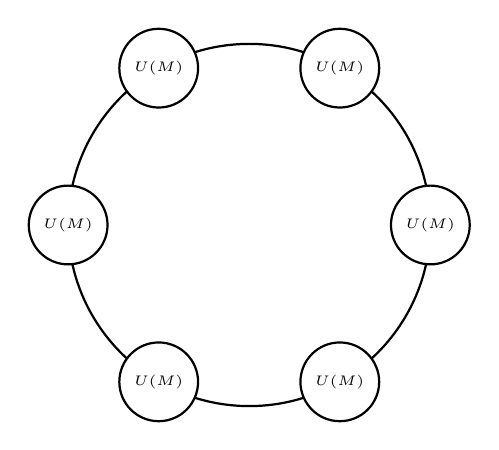
\begin{tikzpicture}[square/.style={regular polygon,regular polygon sides=4},thick,inner sep=0.1em]
     \newdimen\R
   \R=2.3cm
   \draw (0,0) circle (\R);
   \foreach \x/\l/\p in
     { 60/{3},
      120/{2},
      180/{1},
      240/{6},
      300/{5},
      360/{4}
     }
     \node[circle,draw,minimum size=1cm,fill=white] at (\x:\R) {\tiny $U(M)$};
\end{tikzpicture}
  \caption{\it 5d $\N=1$ necklace quiver $\mathcal{N}_{M,N}$ for $N=6$.}
  \label{fig:Skquiver}
\end{figure}
The surface operator is characterised by the partition $\rho$ \eqref{eqn:partitionM} which specifies the embedding into each factor $\mathbb{Z}_k\hookrightarrow U(M=M_A)$.
We called this resulting theory $\mathcal{N}^{\rho}_{M,N}$. We first briefly review the case without defect before turning to the computation with the defect present.

\subsection{Review of \texorpdfstring{$\mathbb{S}^1\times \mathbb{S}^4$}{S1 x S4} Partition Function for \texorpdfstring{$\mathcal{N}_{M,N}$}{N(M,N)}}
We first review the computation for the case without defect, i.e. $k=1$. The partition function is defined as
\begin{equation}\label{eqn:5dindex}
Z\left(s,p,v,\qfk_A\right)=\Tr_{\mathbb{S}^4}\left[(-1)^Fe^{-\beta\delta}s^{-2J_R-2J_R^R}p^{-2J_L}v^{2J_L^R}\prod_{A=1}^N\qfk_A^{K_A}\right]
\end{equation}
where 
\begin{equation}
s:=e^{\iu\beta\epsilon_+/2}\,,\quad p:=e^{\iu\beta\epsilon_-/2}\,,\quad v:=e^{\iu\beta m}\,,
\end{equation}
with $\epsilon_{\pm}=\epsilon_1\pm\epsilon_2$ as before. The trace is taken over the Hilbert space of the theory on $\mathbb{S}^4$ in the radial quantisation. The $\mathcal{N}_{N,M}$ theories have 5d $\mathcal{N}=1$ supersymmetry with supercharges $\Qfive^{\alpha \dot a}$, $\widetilde{\Qfive}^{\dot\alpha \dot a}$. 
We compute the partition function with respect to $\widetilde{\Qfive}:=\widetilde{\Qfive}^{\dot1\dot2}$ and in the radial quantisation $\widetilde{\Sfive}=\widetilde{\Qfive}^{\dagger}$ its conjugate. 
$Z$ is formally independent of $\beta$ since it receives contributions only from those states which satisfy
\begin{equation}\label{eqn:BPS}
\delta:=\left\{\widetilde{\Qfive},\widetilde{\Sfive}\right\}=E-2J_R-3J_R^R=0\,,
\end{equation}
$\qfk_A$ are fugacities for the topological $U(1)$'s associated to the conserved currents
\begin{equation}
\ast_5 J_A=\frac{1}{4\pi^2}F_A\wedge F_A
\end{equation}
corresponding to each gauge node. $Z$ can be computed from localisation, which we review in Appendix \ref{app:SCIrev}, and takes the following form
\begin{equation}\label{eqn:5dindexgeneric}
Z=\oint\prod_{A=1}^N\left[da_A\right]Z_{\text{south}}Z_{\text{north}}=\oint\prod_{A=1}^N\left[da_A\right]\left|Z_{\text{Nek}}\right|^2
\end{equation} 
where
\begin{equation}
M_{A}![da_A]=\Delta(a_A)\prod_{n=1}^{M_A}\frac{d a_{A,n}}{2\pi}=\prod_{n=1}^{M_A}\frac{d a_{A,n}}{2\pi}\prod_{m\neq n}2\sin\frac{a_{A,n}-a_{A,m}}{2}
\end{equation}
is the Haar measure for $U(M_A=M)$. Here $Z_{\text{Nek}}$ is the Nekrasov partition function for self-dual instantons
\begin{equation}
Z_{\text{Nek}}=Z_{\text{south}}=Z^{\text{1-loop}}_{\text{south}}Z_{\text{inst}}\,.
\end{equation}
\subsubsection{1-Loop Contributions}
The one-loop contributions factor into contributions from vector and hypermultiplets
\begin{equation}
Z^{\text{1-loop}}_{\text{south}}=Z^{\text{1-loop}}_{\text{south},\text{vec}}Z^{\text{1-loop}}_{\text{south},\text{hyp}}\,.
\end{equation}
Let us begin with the vector multiplets.
\paragraph{Vector Multiplet Contributions} 
The 1-loop contribution for the vectors given by expansion of the equivariant index \eqref{eqn:indexsouth}. At the south pole we should take $|e^{\iu\epsilon_1}|,|e^{\iu\epsilon_2}|>1$ hence 
\begin{equation}
\begin{aligned}
\tilde{Z}=\prod_{p\in\mathbb{Z}}\prod_{\mu,\nu=0}^{\infty}&\prod_{A=1}^N\prod_{n\neq m}\left\{\left[\frac{2\pi p}{\beta}+\mu\epsilon_1+\nu\epsilon_2+\frac{a_{A,n}-a_{A,m}}{\beta}\right]^{\frac{1}{2}}\right.\\
&\times\left.\left[\frac{2\pi p}{\beta}+(\mu+1)\epsilon_1+(\nu+1)\epsilon_2+\frac{a_{A,n}-a_{A,m}}{\beta}\right]^{\frac{1}{2}}\right\}\,.
\end{aligned}
\end{equation}
The partition function is defined only up to an overall constant and $\sim$ denotes that the divergent factor, which is independent of all chemical potentials, has been removed. 
\begin{equation}
\begin{aligned}
\tilde{Z}\sim&\prod_{\mu,\nu=0}^{\infty}\prod_{A=1}^N\prod_{n\neq m}\left\{\sin\left[\frac{ a_{A,n}- a_{A,m}- \mu\beta\epsilon_1- \nu\beta\epsilon_2}{2}\right]^{\frac{1}{2}}\right.\\
&\times\left.\sin\left[\frac{ a_{A,n}- a_{A,m}-(\mu+1)\beta\epsilon_1-(\nu+1)\beta\epsilon_2}{2}\right]^{\frac{1}{2}}\right\}\\
=&e^{\frac{\beta\epsilon_+E_0}{2}}\left(\prod_{A=1}^N\Delta(a_A)^{\frac{1}{2}}\right)\PE\left[-\frac{s(p+p^{-1})}{2(1-sp)(1-sp^{-1})}\sum_{A=1}^N\sum_{n\neq m}\frac{x_{A,n}}{x_{A,m}}\right]\\
\equiv& \left(\prod_{A=1}^N\Delta(a_A)^{\frac{1}{2}}\right)Z^{\text{1-loop}}_{\text{south},\text{vec}}\,.
\end{aligned}
\end{equation}
In the final line $E_0$ is the Casimir energy. We also defined $x_{A,n}:=e^{\iu a_{A,n}}$ and then factored out the Vandermonde determinants 
\begin{equation}
\Delta(a_A)=\exp\left(-\sum_{l=1}^{\infty}\frac{1}{l}\sum_{n\neq m}\left(e^{\iu a_{A,n}-\iu a_{A,m}}\right)^{l}\right)=\PE\left[-\sum_{n\neq m}x_{A,n}x_{A,m}^{-1}\right]\,,
\end{equation}
which arises from the zero modes of the vector multiplets. Moreover, the vector contribution is invariant under conjugation so
\begin{equation}
Z^{\text{1-loop}}_{\text{north},\text{vec}}=\left(
Z^{\text{1-loop}}_{\text{south},\text{vec}}\right)^*=
Z^{\text{1-loop}}_{\text{south},\text{vec}}\,.
\end{equation}
\paragraph{Hypermultiplet Contributions}
Here we compute the contributions from hypermultiplets. The hypermultiplet contains complex scalars $\varphi^{\dot a}$ and fermions $\psi$ plus their conjugates. Note $\varphi^{\dot1},\varphi^{\dot2}$ are identified with $X_{89}^{\dagger}$, $X_{710}$ and hence have charges $+\frac{1}{2}$ under $J_L^R$. The multiplets live in bifundamental representations of $SU(M_{A})\times SU(M_{A+1})$.
\begin{table}
\centering
 \begin{tabular}{|c|c|c|c|c|c|c|} 
 \hline
Letter & $E$& $J_R$ &$J_R^R$& $J_L$&$J_L^R$& Index\\\hline
\hline
$\varphi^{\dot2}$ &$3/2$ & $0$& $+1/2$&$0$& $+1/2$ & $sv$\\\hline
$\bar{\varphi}^{\dot2}$ &$3/2$ & $0$& $+1/2$&$0$& $-1/2$ & $sv^{-1}$\\\hline
\hline
$\partial_{1\dot1}$ &$1$ &$+1/2$ & $0$ &$+1/2$&$0$&$sp$\\\hline
$\partial_{2\dot1}$ &$1$ &$+1/2$ & $0$ & $-1/2$&$0$&$sp^{-1}$\\\hline
\end{tabular}
\caption{\it The letters of the Hypermultiplet with $\delta=0$.}
 \label{tab:hypletters}
\end{table}
Since there are no-zero modes coming from the hypermultiplet its contribution to the index may be computed via letter counting. The contribution to the index from hypermultiplets is given by enumerating all `letters' listed in Table \ref{tab:hypletters}. We may identify the contribution localised at the south pole as coming from a half-hypermultiplet \eqref{eqn:hypindexsouth}
\begin{equation}\label{eqn:hyperpartsouth}
Z^{\text{1-loop}}_{\text{south},\text{hyp}}=e^{\frac{-\beta\epsilon_+E_0}{2}}\PE\left[\sum_{A=1}^N\sum_{n=1}^{M_A}\sum_{m=1}^{M_{A+1}}\frac{sv}{(1-sp)(1-sp^{-1})}x_{A,n}x_{A+1,m}^{-1}\right]\,.
\end{equation}
At the north pole the anti-half-hypermultiplet contribution is localised
\begin{equation}\label{eqn:hyperpartnorth}
Z^{\text{1-loop}}_{\text{north},\text{hyp}}=e^{\frac{-\beta\epsilon_+E_0}{2}}\PE\left[\sum_{A=1}^N\sum_{n=1}^{M_A}\sum_{m=1}^{M_{A+1}}\frac{sv^{-1}}{(1-sp)(1-sp^{-1})}x_{A,n}^{-1}x_{A+1,m}\right]\,.
\end{equation}

\subsubsection{Instanton Contributions}
Recall from the localisation that (anti-)self-dual instantons ($F^-=0$) $F^+=0$ can be localised at (north)south-pole.
The instanton contribution may be computed from equivariant integration over the moduli space $\mathbf{M}_K$ of $K=\sum_AK_A$ $U(M)^N$ instantons. See Sections \ref{Chap:AppInstADHM} \& \ref{sec:intronekpart}.
$\mathbf{M}_K$ carries a torus action $T:=T^3_{\epsilon_1,\epsilon_2,m}\times T(U(N))^M\acts \mathbf{M}_K$ where $T(G)$ denotes a maximal torus of $G$. $\epsilon_1$, $\epsilon_2$, $m$ and $\vec{a}\in\mathfrak{t}$ . 
The instanton moduli space $\mathbf{M}_K$ may be described as a algebraic variety using the ADHM construction \cite{Atiyah:1978ri}. The fixed points of the torus action $T$ on the ADHM data are labelled by $N$ $M$-tuples of Young diagrams $\vec{\mu}_A$ such that $|\vec{\mu}_A|=K_A$. 
The character of the tangent space $T\mathbf{M}_K$ at the fixed point labelled by a set of $M$-tuples $\{\vec{\mu}_A\}$ is then
\begin{equation}
\chi_{\{\vec{\mu}_A\}}\left(T\mathbf{M}_K\right):=\chi_{\{\vec{\mu}_A\}}^{\text{vec}}+\chi_{\{\vec{\mu}_A\}}^{\text{hyp}}\,,
\end{equation}
where
\begin{align}
&\chi_{\{\vec{\mu}_A\}}^{\text{vec}}=\sum_{A=1}^N\left(W_{A}^*V_A+e^{\epsilon_+}V_A^*W_A-(1-e^{\epsilon_1})(1-e^{\epsilon_2})V_A^*V_A\right)\mathcal{P}\,,\\
&\begin{aligned}
\chi_{\{\vec{\mu}_A\}}^{\text{hyp}}=-e^{\tilde{m}}\sum_{A=1}^N&\left(W_{A+1}^*V_A+e^{\epsilon_+}V_{A}^*W_{A-1}\right.\\
&\left.-(1-e^{\epsilon_1})(1-e^{\epsilon_2})V_A^*V_{A-1}\right)\mathcal{P}\,.
\end{aligned}
\end{align}
Where $\tilde{m}=m-\frac{\epsilon_+}{2}$ and
\begin{equation}
V_A=\sum_{n=1}^M\sum_{(l,p)\in\mu_{A,n}}e^{a_{A,n}+(1-l)\epsilon_1+(1-p)\epsilon_2}\,,\quad W_A=\sum_{n=1}^Me^{a_{A,n}}\,,
\end{equation}
and the conjugation flips the sign of the exponents. We also added the dressing by momentum factors along the $\mathbb{S}^1$, with radius $r=\beta$
\begin{equation}
\mathcal{P}:=\sum_{t\in\mathbb{Z}}e^{\frac{2\pi t}{r}}\,.
\end{equation}
We have arrived at these expressions in precisely the same way we used in Section \ref{sec:intronekpart}.
Using the identity \eqref{eqn:youngsimp} it can be shown that
\begin{align}
&\chi_{\{\vec{\mu}_A\}}^{\text{vec}}=\sum_{A=1}^N\sum_{n,n'=1}^M\sum_{s\in\mu_{A,n'}}\left(e^{E_{AA,nn'}(s)}+e^{\epsilon_+-E_{AA,nn'}(s)}\right)\mathcal{P}\,,\\
&\chi_{\{\vec{\mu}_A\}}^{\text{hyp}}=\sum_{A=1}^N\sum_{n,n'=1}^M\sum_{s\in\mu_{A,n'}}e^{\tilde{m}}\left(e^{E_{A(A-1),nn'}(s)}+e^{\epsilon_+-E_{A(A+1),nn'}(s)}\right)\mathcal{P}\,,
\end{align}
where, for a box $s=(l,p)$,
\begin{equation}
E_{AB,nn'}(s):=a_{A,n}-a_{B,n'}-(\mu^{\trans}_{B,n';j}-l)\epsilon_1+(\mu_{A,n;i}-p+1)\epsilon_2\,.
\end{equation}
The contribution of the fixed point $\{\vec{\mu}_A\}$ to the instanton partition is obtained from the character by
\begin{equation}\label{eqn:conversionrule}
\chi_{\{\vec{\mu}_A\}}\left(T\mathbf{M}_K\right):=\sum_{i}n_ie^{w_i}\quad \to \quad z_{\vec{\mu}}=\prod_{i}w_i^{-n_i}\,.
\end{equation}
Finally, after applying the infinite product \eqref{eqn:Eulersine} for the sine function, the instanton partition function is given by a weighted sum over all possible $N$-tuples $\vec{\mu}_A$
\begin{equation}
Z_{\text{inst}}\left(\vec{a}_A,m,\epsilon_1,\epsilon_2,\qfk_A,\beta\right)=\sum_{\vec{\mu}_A} \left(\prod_{A=1}^N\qfk_A^{|\vec{\mu}_A|}\right)z_{\{\vec{\mu}_A\}}\left(\vec{a}_A,m,\epsilon_1,\epsilon_2,\beta\right)\,,
\end{equation}
\begin{equation}
\begin{aligned}
z_{\{\vec{\mu}_A\}}=&\prod_{A=1}^N\prod_{n,n'=1}^M\prod_{s\in\mu_{A,n'}}\Bigg\{\\
&\frac{\sin\frac{\beta}{2}\left(E_{A(A-1),nn'}(s)+\tilde{m}\right)\sin\frac{\beta}{2}\left(E_{A(A+1),nn'}(s)-\tilde{m}-\epsilon_+\right)}{e^{\kappa_A\phi_{A,n}(s)}\sin\frac{\beta}{2}E_{AA,nn'}(s)\sin\frac{\beta}{2}\left(E_{AA,nn'}(s)-\epsilon_+\right)}\Bigg\}\,,
\end{aligned}\label{eqn:fpcont}
\end{equation}
where $\tilde{m}:=m-\frac{\epsilon_+}{2}$ we also allowed for non-zero Chern-Simons levels $\kappa_A$ and the function $\phi_{A,n}(s)$ is defined to be
\begin{equation}
\phi_{A,n}(s):=a_{A,n}+\left(l-\frac{1}{2}\right)\epsilon_1+\left(p-\frac{1}{2}\right)\epsilon_2\,.
\end{equation} 

\subsection{\texorpdfstring{$\mathbb{S}^1\times \mathbb{S}^4$}{S1 x S4} Partition Function for \texorpdfstring{$\mathcal{N}^{\rho}_{M,N}$}{Nr(M,N)}}
We now come to the calculation in the presence of the defect. The defect is supported along a codimension 2 hypersurface within $\mathbb{S}^1\times \mathbb{S}^4$. For simplicity we will consider only the following: choose a local coordinate patch $\mathbb{R}^4\iso\mathbb{C}_{\epsilon_1}\times\mathbb{C}_{\epsilon_2}$ parametrised by $(z_1,z_2)$, at the either pole we may choose for a defect of type $\rho$ to be supported along either $\mathbb{S}^1\times\mathbb{C}_{\epsilon_1}$ or $\mathbb{S}^1\times\mathbb{C}_{\epsilon_2}$. Requiring that the defect preserves atleast $\widetilde{\Qfive}=\widetilde{\Qfive}^{\dot1\dot2}$ means we can only choose the latter. Recall that the surface operator is defined by demanding singular behaviour of the gauge fields, in local coordinates let $z_2=re^{\iu\theta}$ then
\begin{equation}
A_{A,\mu}dx^{\mu}+A_{A,5}dx^5\sim\diag\left(\alpha_{A1},\dots,\alpha_{Ak}\right)\iu d\theta\,,
\end{equation}
which breaks the gauge group
\begin{equation}
\prod_{A=1}^NU(M_{A})\to\prod_{A=1}^N\prod_{i=1}^kU(M_{Ai})\,.
\end{equation}
We then compute
\begin{equation}\label{eqn:5dindexdefect}
Z^{\rho}\left(s,p,v,\qfk_{Ai}\right)=\Tr_{\mathbb{S}^4}\left[(-1)^Fe^{-\beta\delta}s^{-2J_R-2J_R^R}p^{-2J_L}v^{2J_L^R}\prod_{A=1}^N\prod_{i=1}^k\qfk_{Ai}^{K_{Ai}}\right]\,.
\end{equation} 
Where 
\begin{equation}
\qfk_{Ai}=\qfk^{\alpha_{Ai}-\alpha_{A(i+1)}}_A\,,\quad i\sim i+k\,. 
\end{equation}
Since the partition function localises on the north and south poles, it is expected that the insertion of a defect at e.g. the south pole does does not affect the contributions localised at the north pole. We hence assume that the index may again be expressed as
\begin{equation}\label{eqn:5dindexgenericdefect}
Z^{\rho}=\int\prod_{A,i}[da_{Ai}]Z^{\rho}_{\text{south}}\left(\vec{a}_{Ai},\epsilon_1,\epsilon_2,m,\qfk_{Ai}\right)Z^{\rho}_{\text{north}}\left(\vec{a}_{Ai},\epsilon_1,\epsilon_2,m,\overline{\qfk}_{Ai}\right)\,.
\end{equation}
In the neighbourhood of the defect we may employ the $\mathbb{Z}_k$ orbifold description of the surface operator at the north and south poles. For example, at the south pole the defect may be effectively described by $\mathbb{C}_{\epsilon_1}\times\mathbb{C}_{\epsilon_2}/\mathbb{Z}_k$ acting by
\begin{equation}
\mathbb{Z}_k:(z_1,z_2)\mapsto(z_1,\omega_kz_2)
\end{equation}
in order to preserve supersymmetry we also twist the coordinate $U(1)_{\epsilon_2}$ action on $z_2$ with a $U(1)\subset SU(2)$ of the R-symmetry group as in \eqref{eqn:orbaction}. The $\mathbb{Z}_k$ actions commute with the localising supercharge. We employ the similar description of the surface defect at the north pole. 
%
\subsubsection{1-Loop Contributions}
To compute the 1-loop factors in the presence of the defect we employ the orbifold description of the defect. Since the $\mathbb{Z}_k$ actions commute with \eqref{eqn:locsusycharge} the vector multiplet 1-loop contributions at north \& south pole may be obtained by computing the equivariant index of the $\mathbb{Z}_k$ invariant part of the complexes \eqref{eqn:northcmplx} \& \eqref{eqn:southcmplx} respectively. The 1-loop contributions from the hypermultiplet may be obtained in a similar fashion, by restricting to the $\mathbb{Z}_k$ invariant part of the Dirac complex \eqref{eqn:Diraccmplx}. Equivalently, we may also count only $\mathbb{Z}_k$ invariant letters of Table \ref{tab:hypletters}.
\paragraph{Vector Multiplets}
For concreteness let us describe the defect $\rho$ at the south pole. In terms of $\mathbb{C}^2$ local coordinates $(z_1,z_2)$ the orbifold acts by
\begin{equation}\label{eqn:orbaction1}
\mathbb{Z}_k:\epsilon_2\mapsto \epsilon_2+\frac{2\pi\iu}{\beta k}j\,,\quad a_{Ai,n}\mapsto a_{Ai,n}+\frac{2\pi\iu }{k}j\left(i+\frac{1}{2}\right)\,.
\end{equation}
Keeping only orbifold invariant factors leads to the modified 1-loop determinant
\begin{equation}\label{eqn:orbvec1loopsin}
\begin{aligned}
&\widetilde{Z}^{\rho}(\epsilon_1,\epsilon_2,\vec{a}_{Ai})=\left(\prod_{A=1}^N\prod_{i=1}^k\Delta(a_{Ai})^{\frac{1}{2}}\right)Z_{\text{south},\text{vectors}}^{\text{1-loop},\rho}(\epsilon_1,\epsilon_2,\vec{a}_{Ai})\\
&=\prod_{\mu,\nu=0}^{\infty}\prod_{A=1}^N\Bigg\{\prod_{i=1}^k\prod_{n\neq m}\Bigg(\sin\left[\frac{ a_{Ai,n}- a_{Ai,m}- \mu\beta\epsilon_1- \nu k\beta \epsilon_2}{2}\right]^{\frac{1}{2}}\\
&\times\sin\left[\frac{ a_{A,n}- a_{A,m}-(\mu+1)\beta\epsilon_1-(\nu+1)k\beta \epsilon_2}{2}\right]^{\frac{1}{2}}\Bigg)\prod_{i\neq j}\prod_{n,m=1}^{M_{Ai},M_{Aj}}\Bigg(\\
&\times\sin\left[\frac{ -a_{Ai,n}+ a_{Aj,m}- (1+\mu)\beta\epsilon_1- (\nu k+[[j-i]])\beta \epsilon_2}{2}\right]^{\frac{1}{2}}\\
&\times\sin\left[\frac{ -a_{Ai,n}+a_{Aj,m}-\mu\beta\epsilon_1-(k\nu+1+[[j-i-1]])\beta \epsilon_2}{2}\right]^{\frac{1}{2}}\Bigg)\Bigg\}
\end{aligned}
\end{equation}
where, as before,  we dropped the overall, fugacity independent, infinite constant and
\begin{equation}\label{eqn:brack}
\left[\left[x\right]\right]:=\left\{
\#\in\mathbb{Z} \,\middle|\text{ $0\leq \#\leq k-1$ and $\#=x\bmod k$}\right\}=\left|x-k\left\lfloor \frac{x}{k}\right\rfloor\right|\,.
\end{equation} 
We may also write \eqref{eqn:orbvec1loopsin} more compactly in terms of the Pletystic exponent
\begin{equation}
\begin{aligned}
&Z_{\text{south},\text{vectors}}^{\text{1-loop},\rho}(\epsilon_1,\epsilon_2,\vec{a}_{Ai})=e^{\frac{\beta\epsilon_+E^{\mathbb{Z}_k}_0}{4}} \times\\
&\PE\left[-\sum_{i,j=1}^k\frac{e^{\iu\beta \epsilon_1}e^{\iu\beta [[j-i]]\epsilon_2}+e^{\iu\beta\left([[j-1-i]]+1\right)\epsilon_2}}{2(1-e^{\iu\beta\epsilon_1})(1-e^{\iu\beta k\epsilon_2})}\sum_{A=1}^N\sum^{M_{Ai},M_{Aj}}_{\substack{n,m=1\\\text{\tiny $n\neq m$ if $i=j$}}}\frac{e^{\iu a_{Ai,n}}}{e^{\iu a_{Aj,m}}}\right]\,.
\end{aligned}
\end{equation}
At the north pole, the conribution is the same and $
Z^{\text{1-loop},\rho}_{\text{south},\text{vec}}=
Z^{\text{1-loop},\rho}_{\text{north},\text{vec}}$ for any $\rho$.
\paragraph{Hypermultiplets} 
For the hypermultiplet, in addition to the action \eqref{eqn:orbaction1} there is also the additional action on the mass parameter 
\begin{equation}\label{eqn:massparamorbact}
\mathbb{Z}_k:m\mapsto m-\frac{2\pi\iu}{\beta k}\frac{j}{2}\,.
\end{equation}
In the presence of the defect at the south pole we have
\begin{equation}
\begin{aligned}
&Z_{\text{south},\text{hypers}}^{\text{1-loop},\rho}\sim \\&\PE\left[\sum_{A=1}^N\sum_{i,j=1}^k\sum_{n,m=1}^{M_{Ai},M_{(A+1)j}}\frac{e^{\iu\beta\frac{\epsilon_+}{2}}e^{\iu\beta m}e^{\iu\beta[[j-i]] \epsilon_2}e^{\iu a_{Ai,n}-\iu a_{(A+1)j,m}}}{(1-e^{\iu\beta\epsilon_1})(1-e^{\iu\beta k\epsilon_2})}\right]\,.
\end{aligned}
\end{equation}
On the other hand, at the north pole
\begin{equation}
\begin{aligned}
&Z_{\text{north},\text{hypers}}^{\text{1-loop},\rho}\sim \\& \PE\left[\sum_{A=1}^N\sum_{i,j=1}^k\sum_{n,m=1}^{M_{Ai},M_{(A+1)j}}\frac{e^{\iu\beta\frac{\epsilon_+}{2}}e^{-\iu\beta m}e^{-\iu\beta[[j+1-i]] \epsilon_2}e^{-\iu a_{Ai,n}+\iu a_{(A+1)j,m}}}{(1-e^{\iu\beta\epsilon_1})(1-e^{\iu\beta k\epsilon_2})}\right]\,.
\end{aligned}
\end{equation}
Because the conjugation exchanges $m\to-m$, in the presence of defects \newline$Z_{\text{north},\text{hypers}}^{\text{1-loop},\rho}\neq \left(Z_{\text{south},\text{hypers}}^{\text{1-loop},\rho}\right)^*$.
\subsubsection{Instanton Contributions}\label{sec:s1s4surfinst}
After the orbifolding the character of the tangent space $T\mathbf{M}_K$ at the fixed point labelled by a set of $M$-tuples $\{\vec{\mu}_{A}\}$ with $\{\vec{\mu}_{A}\}=\{\mu_{Ai,n}\}$ with $A=1,\dots,N$, $i=1,\dots,k$, $n=1,\dots, M_{Ai}$ is given by restricting to the fixed point of the action
\eqref{eqn:orbaction1}, \eqref{eqn:massparamorbact}. It is given by
\begin{equation}\label{eqn:indorb}
\chi^{\text{orb}}_{\{\vec{\mu}_A\}}\left(T\mathbf{M}_K\right):=\chi_{\{\vec{\mu}_A\}}^{\text{vec},\text{orb}}+\chi_{\{\vec{\mu}_A\}}^{\text{hyp},\text{orb}}\,,
\end{equation}
where,
\begin{equation}
\begin{aligned}\chi_{\{\vec{\mu}_A\}}^{\text{vec},\text{orb}}=\sum_{A=1}^N\sum_{i=1}^k&\left(W_{A,i}^*V_{A,i}+e^{\epsilon_+}V_{A,i-1}^*W_{A,i}-(1-e^{\epsilon_1})V_{A,i}^*V_{A,i}\right.\\
&\left.+(1-e^{\epsilon_1})e^{\epsilon_2}V_{A,i-1}^*V_{A,i}\right)\mathcal{P}\,,
\end{aligned}
\end{equation}
\begin{equation}
\begin{aligned}
\chi_{\{\vec{\mu}_A\}}^{\text{hyp},\text{orb}}=&-e^{\tilde{m}}\sum_{A=1}^N\sum_{i=1}^k\left(W_{A+1,i+1}^*V_{A,i}+e^{\epsilon_+}V_{A,i}^*W_{A-1,i}\right.\\
&\left.-(1-e^{\epsilon_1})V_{A,i+1}^*V_{A-1,i}+(1-e^{\epsilon_1})e^{\epsilon_2}V_{A,i}^*V_{A-1,i}\right)\mathcal{P}\,.\end{aligned}
\end{equation}
Where
\begin{equation}
V_{A,i}=\sum_{j=1}^k\sum_{n=1}^{M_{A(i-j+1)}}\sum_{(l,kp+j)\in\mu_{A(i-j+1),n}}e^{v_{A,ij,n}(l,p)}\,,\quad W_{A,i}=\sum_{n=1}^{M_{Ai}}e^{a_{Ai,n}}\,,\label{eqn:simpleinstform}
\end{equation}
\begin{equation}
v_{A,ij,n}(l,p):=a_{A(i-j+1),n}+(1-l)\epsilon_1+(1-pk-j)\epsilon_2+k\left\lfloor\frac{i-j}{k}\right\rfloor\epsilon_2
\end{equation}
and the conjugation flips the sign of the exponents. We also added the dressing by momentum factors along the $\mathbb{S}^1$. Converting the character using \eqref{eqn:conversionrule} gives
\begin{equation}
z^{\text{orb}}_{\{\vec\mu_A\}}=z^{\text{vec},\text{orb}}_{\{\vec\mu_A\}}z^{\text{hyp},\text{orb}}_{\{\vec\mu_A\}}\,,
\end{equation}
\begin{equation}
\begin{aligned}
&z^{\text{vec},\text{orb}}_{\{\vec\mu_A\}}=\prod_{A,i,j,n,n'}\Bigg\{\prod_{(l,kp+j)\in\mu_{A(i-j+1),n}}\sin\frac{r}{2}\left(v_{A,ij,n}(l,p)-a_{Ai,n'}\right)\\
&\times\prod_{(l,kp+j)\in\mu_{A(i-j+1),n}}\sin\frac{r}{2}\left(-v_{A,ij,n}(l,p)+a_{A(i+1),n'}+\epsilon_+\right)\\
&\times\prod_{j'}\prod_{\substack{(l,kp+j)\in\mu_{A(i-j+1),n}\\(l',kp'+j')\in\mu_{A(i-j'+1),n'}}}\frac{\sin\frac{r}{2}\left(v_{A,ij,n}(l,p)-v_{A,ij',n'}(l',p')+\epsilon_1\right)}{\sin\frac{r}{2}\left(v_{A,ij,n}(l,p)-v_{A,ij',n'}(l',p')\right)}\\
&\times\prod_{j'}\prod_{\substack{{(l,kp+j)\in\mu_{A(i-j+1),n}}\\(l',kp'+j')\in\mu_{A(i-j'),n'}}}\frac{\sin\frac{r}{2}\left(v_{A,ij,n}(l,p)-v_{A,(i-1)j',n'}(l',p')+\epsilon_2\right)}{\sin\frac{r}{2}\left(v_{A,ij,n}(l,p)-v_{A,(i-1)j',n'}(l',p')+\epsilon_+\right)}\Bigg\}\,,
\end{aligned}
\end{equation}
\begin{equation}
\begin{aligned}
&z^{\text{hyp},\text{orb}}_{\{\vec\mu_A\}}=\prod_{A,i,j,n,n'}\Bigg\{\prod_{(l,kp+j)\in\mu_{A(i-j+1),n}}\frac{1}{\sin\frac{r}{2}\left(v_{A,ij,n}(l,p)-a_{(A-1)(i-1),n'}+\tilde{m}\right)}\\
&\times\prod_{(l,kp+j)\in\mu_{A(i-j+1),n}}\frac{1}{\sin\frac{r}{2}\left(-v_{A,ij,n}(l,p)+a_{(A+1)i,n'}+\tilde{m}+\epsilon_+\right)}\\
&\times\prod_{\substack{j'\\(l,kp+j)\in\mu_{(A-1)(i-j+1),n}\\(l',kp'+j')\in\mu_{A(i-j'+2),n'}}}\frac{\sin\frac{r}{2}\left(v_{A-1,ij,n}(l,p)-v_{A,(i+1)j',n'}(l',p')+\tilde{m}\right)}{\sin\frac{r}{2}\left(v_{A-1,ij,n}(l,p)-v_{A,(i+1)j',n'}(l',p')+\frac{\epsilon_-}{2}+m\right)}\\
&\times\prod_{\substack{j'\\(l,kp+j)\in\mu_{(A-1)(i-j+1),n}\\(l',kp'+j')\in\mu_{A(i-j'+1),n'}}}\frac{\sin\frac{r}{2}\left(v_{A-1,ij,n}(l,p)-v_{A,ij',n'}(l',p')+\tilde{m}+\epsilon_+\right)}{\sin\frac{r}{2}\left(v_{A-1,ij,n}(l,p)-v_{A,ij',n'}(l',p')+m-\frac{\epsilon_-}{2}\right)}\Bigg\}\,.
\end{aligned}
\end{equation}
All in all, the instanton partition function with surface operator is given by
\begin{equation}
Z_{\text{inst}}^{\text{orb}}\left(\vec{a}_{Ai},m,\dots;\qfk_{Ai}\right)=\sum_{\vec{\mu}_A} \left(\prod_{A=1}^N\prod_{i=1}^k\qfk_{Ai}^{K_{Ai}(\vec{\mu}_{A})}\right)z^{\text{orb}}_{\{\vec{\mu}_A\}}\left(\vec{a}_{Ai},\dots\right)\,,
\end{equation}
where
\begin{equation}
K_{Ai}=d_{Ai}(\vec{\mu_A})=\sum_{p=1}^{\infty}\sum_{n=1}^{M_{A(i+1-j)}}\mu_{A(i+1-j),n;p}\,.
\end{equation}
A generalisation of this result for generic orbifold action $(z_1,z_2)\mapsto(\omega_k^{q_1}z_1,\omega_k^{q_2}z_2)$ for the case of 5d $\mathcal{N}=1^*$ theory can be found in Appendix \ref{Chap:AppRamInsts}. It would be interesting to investigate whether this result can be used to study the partition functions of 5d theories in the presence of more general defects. 
\subsection{Unrefined Limits for 5d MSYM}
In certain special limits the index without defect \eqref{eqn:5dindex} is known to admit drastic simplifications. We would like to investigate whether this holds true also when one considers the case with defect \eqref{eqn:5dindexgeneric}.

We restrict ourselves to the case $N=1$ then we have a theory of a single $U(M)$ $\mathcal{N}=1$ vector multiplet with an adjoint hypermultiplet, i.e. the $U(M)$ $\mathcal{N}=2$ theory. This theory has additional supersymmetry, namely 16 supercharges $\Qfive^{\alpha a}$, $\widetilde{\Qfive}^{\dot\alpha \dot a}$; aswell as $\Qfive^{\alpha \dot a}$ and $\widetilde{\Qfive}^{\dot\alpha a}$ from before.
In particular, $\widetilde{\Qfive}^{\dot1a}$ commute with the distinguished supercharge $\widetilde{\Qfive}=\widetilde{\Qfive}^{\dot1\dot2}$.
Moreover, those preserved by the $\epsilon_2$-plane defects are
\begin{equation}
\widetilde{\Qfive}^{\dot1\dot2}\,,\quad \widetilde{\Qfive}^{\dot2\dot1}\,,\quad \widetilde{\Qfive}^{\dot12}\,,\quad \widetilde{\Qfive}^{\dot21}\,,\quad \Qfive^{12}\,,\quad \Qfive^{21}\,,\quad \Qfive^{1\dot2}\,,\quad \Qfive^{2\dot1}\,.
\end{equation}
We can consider some unrefined limits of the index \eqref{eqn:5dindex}. 
\subsubsection{\boldmath $2m=-\epsilon_+$}
The first one we consider is $s=v^{-1}$ or $2m=-\epsilon_+$. In this limit the index \eqref{eqn:5dindexgeneric} becomes
\begin{equation}\label{eqn:12BPS}
Z^{\rho}\left(s,p,s^{-1},\qfk_i\right)=\Tr_{\mathbb{S}^4}\left[(-1)^Fe^{-\beta\delta}s^{-2J_R-2J_R^R-2J_L^R}p^{-2J_L}\prod_{i=1}^k\qfk^{K_i}_i\right]\,.
\end{equation}
In this limit the index is, atleast, a $\frac{1}{4}$-BPS object annihilated by both $\widetilde{\Qfive}$ and $\widetilde{\Qfive}^{\dot12}$ which also has $E-2J_R-3J_R^L=0$, implying that this limit of the index recieves non-zero contributions only from states with $J_L^R=J_R^R$.

\paragraph{Without Defect}
Let us first consider the case without defect. We consider the specialisation of to $2m=-\epsilon_+$. 
In this case, one can check that the perturbative contributions receive large amounts of cancellations and 
\begin{equation}
\Delta(a)Z^{\text{1-loop}}_{\text{south},\text{vec}}Z^{\text{1-loop}}_{\text{north},\text{vec}}Z^{\text{1-loop}}_{\text{south},\text{hyp}}Z^{\text{1-loop}}_{\text{north},\text{hyp}}\to1
\end{equation}
One can also easily see from \eqref{eqn:fpcont} that the contribution for each instanton fixed point is simply $z_{\vec\mu}=1$. It is particularly simple to see by realising that, in this limit, $\chi_{\{\vec{\mu}_A\}}^{\text{vec}}=-\left(\chi_{\{\vec{\mu}_A\}}^{\text{hyp}}\right)^*$. Therefore the instanton partition function is simply counting the number of fixed points
\begin{equation}
Z_{\text{inst}}\to\sum_{\vec{\mu}}\qfk^{|\vec{\mu}|}=\prod_{n=1}^{\infty}\frac{1}{(1-\qfk^n)^{M}}=\PE\left[M\frac{\qfk}{1-\qfk}\right]\,.
\end{equation}
The total partition function \eqref{eqn:12BPS} is then simply
\begin{equation}
Z(s,p,s^{-1},\qfk)=\oint\left[da\right]\left|\PE\left[M\frac{\qfk}{1-\qfk}\right]\right|^2=\left|\left(\qfk;\qfk\right)^M\right|^{2}\,.
\end{equation} 

\paragraph{With Defect}
We now consider the limit in the presence of the defects. It is not too hard to again show that
\begin{gather}
\left(\prod_{i=1}^k\Delta(a_i)\right)Z^{\text{1-loop},\rho}(\epsilon_1,\epsilon_2,m=-\frac{\epsilon_+}{2},\vec{a}_{i})=1\\
z^{\text{orb}}_{\{\vec{\mu}\}}\left(\vec{a}_i,m=\pm\frac{\epsilon_+}{2},\epsilon_1,\epsilon_2,\beta\right)=1
\end{gather}
due to cancellations between vector and hypermultiplets. 
The instanton piece simply counts the number of fixed points
\begin{equation}
\begin{aligned}
&Z_{\text{inst}}^{\text{orb}}\left(\vec{a}_i,m=-\frac{\epsilon_+}{2},\epsilon_1,\epsilon_2,\qfk_{i},\beta\right)=\sum_{\vec{\mu}_A} \left(\prod_{i=1}^k\qfk_{i}^{d_{i}(\vec{\mu})}\right)\cdot1\\
&=(\qfk;\qfk)^{-M}\prod_{i=1}^k\prod_{p=1}^{\infty}\left(1-\prod_{j=1}^{i+p-1}\qfk_j\right)^{-M_i}\\
&=\PE\left[M\frac{\qfk}{1-\qfk}+\sum_{i=1}^k\sum_{j=i+1}^{k}M_i\frac{\prod_{p=i}^j\qfk_p}{1-\qfk}+\sum_{i=2}^k\sum_{j=1}^{i-1}M_i\frac{\qfk\prod_{p=i}^j\qfk_p}{1-\qfk}\right]\,,
\end{aligned}
\end{equation}
the first equality was given in \cite{Kanno:2011fw} and the second conjectured in \cite{Bullimore:2014upa}.
Therefore, in this limit, the partition function with defects at north and south poles reduces to
\begin{equation}
\begin{aligned}
&Z^{\rho}(s,p,s^{-1},\qfk_{i})=\\
&\left|\PE\left[M\frac{\qfk}{1-\qfk}+\sum_{i=1}^k\sum_{j=i+1}^{k}M_i\frac{\prod_{p=i}^j\qfk_p}{1-\qfk}+\sum_{i=2}^k\sum_{j=1}^{i-1}M_i\frac{\qfk\prod_{p=i}^j\qfk_p}{1-\qfk}\right]\right|^2
\end{aligned}
\end{equation}
\subsubsection{\boldmath $2m=-\epsilon_-$}
We can also consider the limit $v=p^{-1}$ or $2m=-\epsilon_-$. In this limit the index becomes
\begin{equation}
Z^{\rho}\left(s,p,p^{-1},\qfk_i\right)=\Tr_{\mathbb{S}^4}\left[(-1)^Fe^{-\beta\delta}s^{-2J_R-2J_R^R}p^{-2J_L-2J_L^R}\prod_{i=1}^k\qfk_i^{K_i}\right]
\end{equation}
\paragraph{Without Defect}
As before, we again consider the case without any defect. For the perturbative piece, is it simple to show that, for $v=p^{-1}$
\begin{equation}
Z^{\text{1-loop}}_{\text{south}}Z^{\text{1-loop}}_{\text{north}}=\PE\left[M\frac{sp+sp^{-1}}{(1-sp)(1-sp^{-1})}\right]
\end{equation}
Moreover, one can show, for the instanton piece that for $|\vec{\mu}|>0$
\begin{equation}
z_{\{\vec{\mu}\}}\left(\vec{a}_i,m=\pm\frac{\epsilon_-}{2},\epsilon_1,\epsilon_2,\beta\right)\equiv0\,.
\end{equation}
Therefore, in this limit, the partition function simply becomes
\begin{equation}
Z^{\rho}\left(s,p,p^{-1},\qfk_i\right)=\PE\left[M\frac{sp+sp^{-1}}{(1-sp)(1-sp^{-1})}\right]\,.
\end{equation}
\paragraph{With Defect}
In the case of inserting the defect, for $m=-2\epsilon_-$ the perturbative piece takes on a similar form
\begin{equation}
Z_{\text{south}}^{\text{1-loop},\rho}Z_{\text{north}}^{\text{1-loop},\rho}=\PE\left[M\frac{sp+s^kp^{-k}}{(1-sp)(1-s^kp^{-k})}\right]\,,
\end{equation}
with $M=\sum_{i=1}^kM_i$.
It was also shown in \cite{Bullimore:2014upa} that, for the ramified instanton partition function, for $|\vec{\mu}|\neq0$
\begin{equation}
z^{\rho}_{\{\vec{\mu}\}}\left(\vec{a}_i,m=\pm\frac{\epsilon_-}{2},\epsilon_1,\epsilon_2,\beta\right)\equiv0\,.
\end{equation}
and therefore, the partition function in the precense of the defects is
\begin{equation}
Z^{\rho}\left(s,p,p^{-1},\qfk_i\right)=\PE\left[M\frac{sp+s^kp^{-k}}{(1-sp)(1-s^kp^{-k})}\right]\,.
\end{equation}

\section{Conclusions}
We have computed the elliptic genus partition functions of the self-dual strings of $\mathcal{N}=(1,0)$ theories associated to $M$ M5-branes on $A_{N-1}$ singularities in the precense of codimension two surface defects labelled by partitions $\rho_A=[M_{A1},\dots,M_{Ak}]$. These BPS strings capture (up to a `perturbative' pre-factor) the states contributing to the $\mathbb{S}^4\times T^2$ partition function of the 6d theory. So called `minimal' defects of type $\rho=[1,\dots,1,(M-p)]$ have been studied from the point of view of topological strings in \cite{Mori:2016qof,Iqbal:2012xm,Vafa:2012fi,Taki:2010bj}. Our method allows straightforward generalisation to obtain the partition functions for any choice of embedding $\rho$'s, which engineer the generic GW-surface operators. The relation between M-strings and refined topological string partition function in the presence of a defect of type $2=1+1$ has been studied in \cite{Mori:2016qof}. It is therefore expected that our M-strings computation captures the information about the refined topological string partiton function for the M-theory background \ref{table:Mtheory}. 

In addition, we have also computed the $\mathbb{S}^4\times \mathbb{S}^1$ partition functions for the 5d $\mathcal{N}_{n,m}$ theories in the presence of $\frac{1}{2}$-BPS codimension two defect operators labelled by $\rho$ inserted at the north and south poles.
\end{document}
